\documentclass[12pt,a4paper]{article}

\usepackage{geometry}
\geometry{
    left=2cm, 
    right=2cm,
    top=3cm,  
    bottom=2cm
}

\usepackage[english,spanish]{babel}
\usepackage[utf8]{inputenc}
\usepackage{amsmath}

\usepackage{graphicx}
\usepackage{wrapfig}
\usepackage{makecell}

\usepackage{booktabs}
\usepackage{enumitem}
\usepackage{xcolor}


\usepackage{csquotes}
\usepackage{hyperref}
\usepackage[style=ieee]{biblatex}
\addbibresource{referencias.bib}

\usepackage{setspace}
\setstretch{1.25}
\setlength{\parindent}{0pt}

\begin{document}
    \begin{titlepage}
        \begin{minipage}[c]{0.1\textwidth}
            
\includegraphics[width=\textwidth]{Resources/logo_unam.jpg}
        \end{minipage}
        \begin{minipage}{0.8\textwidth}
            \centering
            {\Large\textbf{Universidad Nacional Autónoma de México}\\}
            {\large\textbf{Escuela Nacional de Estudios Superiores\\\underline{Unidad Morelia}}}
        \end{minipage}
        \begin{minipage}[c]{0.1\textwidth}
            
\includegraphics[width=\textwidth]{Resources/logo_enes.jpg}
        \end{minipage}
        \vspace{3cm}

        \centering
        {\large{Reporte Final\\}}
        {\Large\textbf{Análisis de Valores Nutricionales por Tipo de Dieta}}
        \vspace{2cm}

        {{PRESENTA:\\}}
        {\large\textbf{Alexis Uriel Aguilar Uribe}}
        \vspace{1cm} 

        {{PROFESORES:\\}}
        {\large\textbf{Dra.\ María Del Río Francos}}\\
        {\large\textbf{Dr.\ César Andrés Torres Miranda}}
        \vspace{2cm}

        {{GRADO\\}}
        {\large\textbf{Licenciatura en Tecnologías para la Información en Ciencias}}
        \vspace{2cm}

        \flushleft{
        {\textbf{Asignatura:\ }Estadística Descriptiva e Inferencial}
        \vspace{2cm}}

        \flushright{
        {\textbf{A:\ }\underline{26 de Mayo del 2025}}}
        \vfill
    \end{titlepage}

\newpage

\tableofcontents

\newpage

\section{Introducción}

    Este trabajo tiene como fin de exponer el proceso llevado a cabo para 
    realizar el análisis estadístico de los valores nutricionales (macronutrientes) 
    que aportan las dietas: \emph{DASH} (Dietary Approaches to Stop Hypertension), 
    \emph{keto}, \emph{mediterránea}, \emph{paleo} (paleolítica) y \emph{vegana}.\\

    Siendo el principal enfoque el responder si hay una diferencia nutricional 
    significativa entre las diferentes dietas. En decir, hacer uso de 
    técnicas de estadística descriptiva e inferencial para probar si existe 
    una diferencia en los aportes nutricionales entre las distintas dietas que 
    están siendo estudiadas. La anterior prueba se basa en recetas de diferentes 
    cocinas a nivel mundial.

    % El propósito final del presenta trabajo es el de crear un modelo estadístico 
    % capaz de categorizar la dieta a la que pertenece una receta en base a los 
    % macronutrientes (carbohidratos, proteínas y grasas) que aporta.

\section{Objetivos Generales}

    Para la realización de lo anterior expuesto, se puntualizan los objetivos del 
    proyecto:
    \begin{itemize}
        \item Realizar de un análisis estadístico de los macronutrientes en las 
        diferentes dietas con el fin de caracterizar sus aportes nutricionales y 
        sus distinciones en las diferentes cocinas.

        \item Conjeturar y probar hipótesis relacionadas a preguntas de interés 
        sobre los aportes nutricionales en cada dieta en base al análisis estadístico. 

        \item Probar si existe una diferencia significativa en los aportes 
        nutricionales entre las diferentes dietas con el fin de probar si cada 
        dieta de estudio es única.
    \end{itemize}

\newpage

\section{Marco Teórico}
    
    La dieta es uno de los principales factores de riesgo de las enfermedades 
    crónicas, y las enfermedades sensibles a la dieta contribuyen en gran medida 
    a los costes sanitarios mundiales. Se han propuesto literalmente miles de 
    \emph{dietas}, que pueden describirse en términos generales como basadas en 
    creencias, en alimentos específicos o en nutrientes; centradas en la 
    pérdida de peso o en el aumento de peso (muscular); dietas de desintoxicación 
    (detox) y dietas diseñadas por razones médicas específicas.\cite{marvastipopular} \\

    Las \emph{dietas de moda} son dietas populares durante un tiempo sin basarse 
    necesariamente en una recomendación dietética estándar. A menudo promueven 
    una pérdida de peso irracionalmente rápida o afirmaciones de salud sin 
    sentido, y se anuncian como dietas que requieren poco esfuerzo por parte de 
    quien las sigue. La promesa de ganancias fáciles, combinada con la presión 
    social para lograr un determinado tipo de cuerpo, puede dejar al público 
    susceptible a afirmaciones infundadas o exageradas.\cite{marvastipopular} \\

    Las dietas estudiadas desde una perspectiva estadística en el presente 
    trabajo, son englobadas en las \emph{dietas de moda}, que a veces son referidas 
    como \emph{dietas sin evidencia científica}. Siendo  la dieta DASH la única 
    que cuenta con algún tipo de fundamento.

    \subsection{DASH (Dietary Approaches to Stop Hypertension)}

        \cite{marvastipopular} La dieta DASH (Enfoques Dietéticos para Detener la 
        Hipertensión) es un patrón dietético diseñado específicamente para ayudar 
        a reducir la presión arterial y promover la salud general del corazón. Hace 
        hincapié en el consumo de una variedad de alimentos ricos en nutrientes, 
        como frutas, verduras, cereales integrales, proteínas magras y productos 
        lácteos bajos en grasa, y en la limitación de la ingesta de sodio, grasas 
        saturadas y azúcares añadidos. 

    \subsection{Dieta Keto}

        \cite{marvastipopular} Una dieta baja en hidratos de carbono (baja en 
        carbohidratos) es un patrón alimentario que restringe la ingesta de 
        carbohidratos, sustituyéndolos normalmente por mayores cantidades de 
        proteínas y grasas. La dieta cetogénica es una forma de dieta baja en 
        carbohidratos con un alto contenido en grasas en relación con la ingesta 
        de proteínas y carbohidratos.\\

        El objetivo de la dieta cetogénica es inducir la cetosis, un estado 
        metabólico que se produce cuando el cuerpo quema grasa para obtener 
        energía en lugar de glucosa, lo que induce la pérdida de peso.

    \subsection{Dieta Mediterránea}

        \cite{marvastipopular} La dieta mediterránea es un patrón alimentario 
        inspirado en los hábitos alimenticios tradicionales de los países 
        situados a orillas del mar Mediterráneo. Se caracteriza por un alto consumo 
        de frutas, verduras, cereales integrales, legumbres, frutos secos y 
        aceite de oliva; un consumo moderado de pescado y aves; y un bajo 
        consumo de carnes rojas, alimentos procesados y dulces.\\

    \subsection{Dieta Paleo (Paleolítica)}

        \cite{marvastipopular} La dieta paleo, también conocida como dieta 
        paleolítica o dieta del hombre de las cavernas, es un enfoque 
        dietético que pretende imitar los hábitos alimentarios de nuestros 
        antiguos antepasados del Paleolítico. \\

        Hace hincapié en el consumo de alimentos integrales y no procesados 
        que habrían estado al alcance de los primeros humanos, como carnes magras, 
        pescado, frutas, verduras, frutos secos y semillas, y excluye los cereales, 
        las legumbres, los productos lácteos, los alimentos procesados y los 
        azúcares añadidos.

    \subsection{Dieta Vegana}

        \cite{marvastipopular} La dieta vegana es un patrón dietético basado en 
        plantas que excluye el consumo de todos los productos de origen animal. Se 
        centra en el consumo de una variedad de alimentos de origen vegetal, como 
        frutas, verduras, cereales legumbres, frutos secos y semillas.\\

        Es importante señalar que, aunque las dietas veganas pueden ser 
        nutricionalmente adecuadas, debe prestarse atención a garantizar una 
        ingesta suficiente de nutrientes esenciales como proteínas, hierro, 
        calcio, vitamina B12 y ácidos grasos omega-3.

\newpage

\section{Presentación de los Datos}

    \subsection{Fuente de Datos}

        El conjunto de datos con el que se está trabajando para este proyecto 
        se encuentran en \cite{dataset_macronutrients}, publicado por la comunidad 
        de Kaggle. Los datos consisten de un conjunto de recetas de diferentes 
        dietas y cocinas, además incluye información de los macronutrientes que 
        aporta cada receta.\\

        \cite{dataset_macronutrients} Aunque en la descripción ni en los metadatos del conjunto de datos se 
        haga mención de las fuentes explícitas de los datos ni el objetivo de 
        esta extracción, sí cuenta con una sección de cómo usar el conjunto de 
        datos, ideas de investigación y reconocimientos.\\

        De los apartados de cómo usar el conjunto de datos e ideas de investigación, 
        se encuentra una idea, implícita, de la información que se quería estudiar. 
        La principal información de interés se vuelve que es: el crear planes 
        alimenticios saludables, ya sea usando las recetas proporcionadas o creando 
        unas nuevas basadas en una dieta y cocina, y el estudiar la relación entre 
        dieta y salud.\\

        Del apartado de reconocimientos, se concluye que las recetas fueron 
        proporcionadas por diferentes creadores de las mismas y demás contribuidores 
        al conjunto de datos. 

    \subsection{Interés del Estudio}

        Se consultó \cite{marvastipopular} en sus 
        capítulos 4 y 8, de donde se proporciona un mejor entendimiento de la 
        importancia de los macronutrientes y una descripción general de las 
        dietas en este trabajo, resultando interesante que en cada dieta se 
        consumen diferentes alimentos y productos con ciertas características 
        para ya sea respetar alguna creencia, fundamento o cuota de macronutrientes. 
        De esto último, proporciona un indicio de que existe una diferencia entre 
        las dietas a nivel de sus aportes nutricionales, por lo tanto, lo que se 
        quiere realizar es probar esta diferencia de manera significativa haciendo 
        uso de la estadística y, en caso de que la haya, mostrar que tanta es ésta 
        diferencia y sus implicaciones.

    \subsection{Variables del Conjunto de Datos}

        El conjunto de datos consta de las siguientes variables. Se menciona su 
        nombre, el tipo de variable y sus valores (en total y únicos):

        \begin{center}
            \begin{tabular}{r|llrr}
                \toprule
                    Variable & Nombre & Tipo & Cantidad de Datos & Valores Únicos\\
                \midrule
                    1 & Diet\_type & Cualitativa Nominal & 7806 & 5 \\
                    2 & Recipe\_name & Cualitativa Nominal & 7806 & 7062\\
                    3 & Cuisine\_type & Cualitativa Nominal & 7806 & 19\\
                    4 & Protein(g) & Cuantitativa Continua & 7806 & 6060\\
                    5 & Carbs(g) & Cuantitativa Continua & 7806 & 6618\\
                    6 & Fat(g) & Cuantitativa Continua & 7806 & 6322\\
                \bottomrule
            \end{tabular}
        \end{center}

        La variable \emph{Recipe\_Name} no es relevante para este trabajo pero figura 
        dentro del dataset. Se hace mención que el conjunto de datos no presenta 
        valores faltantes.

    \subsection{Ejemplo de Registros en el Conjunto de Datos}

        Para ejemplificar como luce el conjunto de datos, se presente 
        una instancia de cada tipo de dieta:

        \begin{center}

            \begin{tabular}{lll}
                \toprule
                    \textbf{Diet\_type} & \textbf{Recipe\_name} & \textbf{Cuisine\_type} \\
                \midrule
                    dash          & Old Fashioned                     & world \\
                    keto          & Keto Egg Drop Soup                & chinese \\
                    mediterranean & Mediterranean Mix                 & mediterranean \\
                    paleo         & Easy Paleo Herb Gravy recipes     & french \\
                    vegan         & Braised Green Beans with Tomatoes & mediterranean \\
                \bottomrule
            \end{tabular}

        \end{center}

        \begin{center}

            \begin{tabular}{rrr}
                \toprule
                    \textbf{Protein(g)} & \textbf{Carbs(g)} & \textbf{Fat(g)} \\
                \midrule
                     0.12 &  9.66 &  0.02 \\
                    21.31 &  9.11 & 60.88 \\
                     8.11 &  9.59 & 14.64 \\
                    23.56 & 39.05 & 42.25 \\
                    17.49 & 77.86 & 70.20 \\
                \bottomrule
            \end{tabular}

        \end{center}

\newpage

\section{Estadística Descriptiva}

    \subsection{Transformación de Datos}\label{subsec:data_trans}

        Debido a que el rango de los valores que pueden tomar los macronutrientes 
        es un rango amplio y que, además, podría dificultar la comparativa a lo largo 
        de las diferentes dietas en sus aportes nutricionales, se decidió que los 
        valores en los macronutrientes sean transformados para trabajar con aportes 
        relativos al total de macronutrientes de cada receta o, equivalentemente, los 
        aportes absolutos de los macronutrientes se normalizaron con la norma $L_1$.\\

        De la anterior transformación, se creó una nuevo atributo que representa el 
        total de macronutrientes que son aportados por cada receta y el rango de los 
        valores que pueden tomar los macronutrientes es $[0,1]$ donde se verifica que 
        la suma de los tres valores (a lo largo de los macronutrientes) es siempre $1$. 
        Este último punto servirá para determinar las distribuciones teóricas de los 
        macronutrientes, en específico los parámetros de la distribución beta que mejor 
        se ajusta a la distribución de cada macronutriente y dieta; esto permite caracterizar 
        las disitrbuciones desde una perspectiva teórico que será relevante para responder 
        la pregunta central de trabajo.\\

        Para el conjunto de datos resultante de la transformación también se les renombraron 
        algunos de sus atributos pero que siguen representando o significando el mismo concepto. 
        De los ejemplos presentando, adquieren la siguiente forma después de transformarlos:

        \begin{center}

            \begin{tabular}{lll}
                \toprule
                    \textbf{Diet\_type} & \textbf{Recipe\_name} & \textbf{Cuisine\_type} \\
                \midrule
                    dash          & Old Fashioned                     & world \\
                    keto          & Keto Egg Drop Soup                & chinese \\
                    mediterranean & Mediterranean Mix                 & mediterranean \\
                    paleo         & Easy Paleo Herb Gravy recipes     & french \\
                    vegan         & Braised Green Beans with Tomatoes & mediterranean \\
                \bottomrule
            \end{tabular}

        \end{center}

        \begin{center}

            \begin{tabular}{rrrr}
                \toprule
                    \textbf{Protein} & \textbf{Carbs} & \textbf{Fat} & \textbf{Total\_Macronutrients} \\
                \midrule
                    0.9857 & 0.0122 & 0.0020 &   9.80 \\
                    0.0997 & 0.2334 & 0.6668 &  91.30 \\
                    0.2965 & 0.2507 & 0.4526 &  32.34 \\
                    0.3724 & 0.2246 & 0.4029 & 104.86 \\
                    0.4703 & 0.1056 & 0.4240 & 165.55 \\
                \bottomrule
            \end{tabular}

        \end{center}

    \subsection{Descripción de los Valores de las Variables}

        Para el presente trabajo se harán uso de las siguientes variables, se 
        acompañan con una descripción de su significado o representación:

        \begin{itemize}[label=\textbullet]

            \item \textbf{Diet\_type}: Variable nominal que representa el tipo de 
            dieta (DASH, keto, mediterránea, paleo, vegana) a la que 
            pertenece una receta. Con esta variable se va permitir estratificar 
            las recetas y estudiarlas de una manera más granular, y para realizar 
            hipótesis sobre lo qué está pasando en una dieta o entre las diferentes dietas.

            \item \textbf{Cuisine\_type}: Variable nominal que representa a qué (estilo 
            de) cocina o región (mexicana, americana, italiana, entre otras) pertenece una 
            receta. Al usarla va a permitir el comparar cómo son las recetas 
            de una dieta en diferentes regiones, y realizar comparativas a lo 
            largo de las dietas.

            \item \textbf{Protein}: Variable continua que representa el 
            porcentaje, respecto al total de macronutrientes, de proteínas que son 
            aportados por una receta.
            \item \textbf{Carbs}: Variable continua que representa el 
            porcentaje, respecto al total de macronutrientes, de carbohidratos que 
            son aportados por una receta.

            \item \textbf{Fat}: Variable continua que representa el 
            porcentaje, respecto al total de macronutrientes, de grasas que son 
            aportados por una receta.

            \item \textbf{Total\_Macronutrients}: Variable continua que representa 
            el total de macronutrientes que son aportados por una receta. Esta variable 
            es auxiliar para la prueba de hipótesis, y no estará presente en la parte 
            del Análisis Estadístico debido a la justificación presentada en 
            subsección anterior~\ref{subsec:data_trans} para la aplicación de la 
            propia transformación.

        \end{itemize}

    \subsection{Visión General de los Datos}
        Primero se presenta un análisis sobre los macronutrientes de 
        las recetas sin estratificarlas según el tipo de dieta.

        \begin{center}
            \begin{tabular}{l|rrr}
                \toprule
                    Medida & Carbs & Protein & Fat \\  
                \midrule
                    Media               & 0.433471 & 0.234762 & 0.331767 \\
                    $Q_1$               & 0.205251 & 0.110188 & 0.184583 \\
                    $Q_2$               & 0.432028 & 0.190931 & 0.314359 \\
                    $Q_3$               & 0.635058 & 0.338059 & 0.464532 \\
                    Desviación Estándar & 0.256032 & 0.163886 & 0.194920 \\
                    Mínimo              & 0.000330 & 0.000000 & 0.000000 \\
                    Máximo              & 1.000000 & 0.887557 & 0.997940 \\
                    Asimetría de Fisher & 0.189556 & 0.922401 & 0.461455 \\
                \bottomrule
            \end{tabular}
        \end{center}

        Debido a que son medidas sobre todos los datos, sin estratificar, 
        se tiene que no hay una referencia de lo que se espera obtener y 
        parte de la información que contienen queda diluida o desvanecida. 
        Esto debido a que las dietas como la vegana es baja en proteínas y 
        la keto en carbohidratos \cite{marvastipopular}, por lo que cualquier 
        suposición no se podría sostener sobre todos las dietas.\\

        Aún así, se reportan bajos valores en proteínas en comparación 
        con los carbohidratos y grasas si se hace uso de la mediana ($Q_2$), 
        dicho así: el cincuenta por ciento de las recetas tienen a lo mucho  
        $19.09\%$ de proteínas, en comparación con el $43.20\%$ de carbohidratos 
        y el $31.43\%$ de grasas. Esto es un indicio de que las recetas, en general, 
        tienden a ser altas en carbohidratos y grasas entre las diferentes dietas y 
        cocinas; mientras que son bajas en proteínas. Este último punto puede ser 
        apoyado si se considera la media de los macronutrientes, que siguen esta 
        tendencia de aportes.\\

        Si se gráfica la distribución de los macronutrientes se tiene que, debido 
        a la asimetría y a la desviación estándar, contienen datos atípicos en proteínas y grasas en una región 
        positiva respecto a la mediana, y esto se relaciona con lo mencionado de que 
        una receta no tiende a un aporte alto de proteínas. Y si se consider el rango 
        intercuartil, se observa que en estos macronutrientes es menor, en comparación, 
        que con el de los carbohidratos, esto muestra como los valores de proteínas y 
        grasas se encuentran concentradas en ciertas regiones en contraste con los posibles 
        valores de los carbohidratos que son más diversos.
        
        \begin{center}
            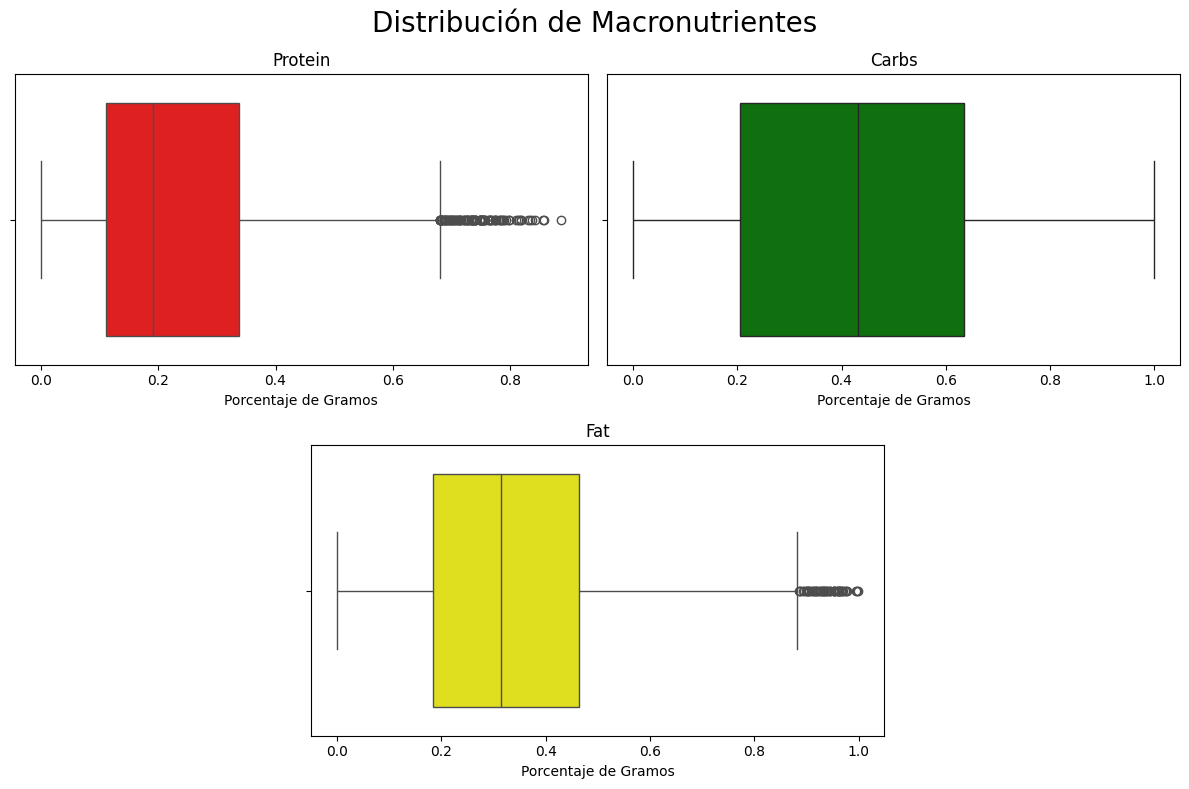
\includegraphics[width=0.90\textwidth]{Resources/2_02_plot_01.png}
        \end{center}

        Debido a que existe la presencia de datos atípicos, lo más adecuado es tratarlos 
        de manera estratificada, por tipo de dieta. Esto debido a que tratarlos de manera 
        general podría evocar que ciertas dietas queden menos representadas en comparación 
        con otras o que incluso se pierda información para consecuentes procesos. Y al 
        tratar los valores atípicos dentro de cada dieta permite reducir el impacto de 
        perder información valiosa y se siga conservando las recetas relevantes para una dieta.\\

        Generando la tabla de contingencia entre tipo de dieta (\emph{Diet\_type}) y de cocina (\emph{Cuisine\_type}), se puede apreciar 
        que dentro del conjunto de datos ciertas cocinas no tienen la suficiente representatividad, 
        provocando que en ciertas dietas tengo nulos registros o una cantidad relativamente pequeña 
        respecto a las demás cocinas dentro de la misma dieta. Destacando como las cocinas kosher y 
        del caribe las que cuentan con la menor cantidad de recetas; y también como la cocina americana 
        es la que mayor representación tiene en el conjunto de datos, seguida de la cocina del mediterráneo 
        donde, como es de esperarse, sus recetas se concentren en su cocina local.
    
        \begin{center}
            \begin{tabular}{l|rrrrr|r}
                \toprule
                & dash & keto & mediterranean & paleo & vegan & Suma Dietas \\
                \midrule
                kosher           & 5    & 0    & 0    & 2    & 0    & 7    \\
                caribbean        & 3    & 7    & 1    & 6    & 1    & 18   \\
                central europe   & 9    & 11   & 1    & 9    & 4    & 34   \\
                japanese         & 9    & 10   & 2    & 5    & 24   & 50   \\
                eastern europe   & 10   & 11   & 3    & 27   & 4    & 55   \\
                middle eastern   & 21   & 17   & 26   & 12   & 15   & 91   \\
                indian           & 20   & 12   & 3    & 9    & 48   & 92   \\
                chinese          & 38   & 38   & 1    & 26   & 17   & 120  \\
                asian            & 24   & 11   & 12   & 12   & 67   & 126  \\
                south american   & 54   & 21   & 10   & 21   & 31   & 137  \\
                south east asian & 31   & 34   & 8    & 29   & 46   & 148  \\
                nordic           & 32   & 35   & 31   & 45   & 9    & 152  \\
                mexican          & 61   & 60   & 17   & 48   & 38   & 224  \\
                british          & 64   & 90   & 4    & 54   & 27   & 239  \\
                world            & 234  & 6    & 6    & 3    & 10   & 259  \\
                french           & 150  & 163  & 61   & 154  & 76   & 604  \\
                italian          & 165  & 234  & 148  & 171  & 81   & 799  \\
                mediterranean    & 176  & 89   & 1274 & 106  & 99   & 1744 \\
                american         & 639  & 663  & 145  & 535  & 925  & 2097 \\
                \midrule
                Suma Cocinas     & 1745 & 1512 & 1753 & 1274 & 1522 & 7806 \\
                \bottomrule
            \end{tabular}
        \end{center}

    \subsection{Estratificación por Tipo de Dieta}

        La variable \emph{Diet\_type} es la principal que se emplea para la 
        estratificación de las recetas, debido a que permite separarlas 
        según una criterio bien definida, a qué dieta pertenecen. Para cada 
        una de las cinco dietas se presentan los datos tabulados de sus 
        medidas de tendencia central y dispersión junto con su histograma 
        de los valores en sus macronutrientes. Por último, se presentan las 
        gráficos de cajas y bigotes de los macronutrientes relevantes por 
        tipo de cocina. 

        \subsubsection{Dieta DASH}

            Una receta de esta dieta tendrá que, en promedio, el $55\%$ de sus 
            macronutrientes son carbohidratos (provenientes de frutas, vegetales 
            y granos enteros); el $25\%$ son grasas que, por su naturaleza, son 
            saludables; y el $20\%$ son proteínas, las cuáles provienen de carnes margas.
            Aunque esta dieta se menciona ser saludable para la salud cardiovascular, 
            no implica que exista un balance o equilibrio en los macronutrientes 
            consumidos por receta.\\

            El cincuenta por ciento de las recetas tienen entre $33\%$ y $76\%$ 
            de carbohidratos en su composición, este fenómeno se puede observar 
            también	en su desviación estándar. Esto implica que los carbohidratos 
            pueden estar en cualquier proporción pero con una tendencia a tener 
            una alta presencia.\\

            Debido a la desviación estándar y rango intercuartil de las proporciones 
            de proteínas y grasas, se tiene que estos macronutrientes se encuentran 
            concentrados en un rango más pequeño de valores en comparación con el 
            fenómeno anterior de la composición de carbohidratos. En específico, el 
            cincuenta por ciento de las recetas tienen entre el $7\%$ y $28\%$ de 
            proteínas y entre $10\%$ y $37\%$ de grasas.

            \begin{center}
                \begin{tabular}{l|lll}
                    \toprule
                        Medida & Carbs & Protein & Fat \\
                    \midrule
                        Media               & 0.549425 & 0.196241 & 0.254334  \\
                        $Q_1$               & 0.331143 & 0.068931 & 0.103381  \\
                        $Q_2$               & 0.555219 & 0.156626 & 0.234742  \\
                        $Q_3$               & 0.757917 & 0.282629 &	0.371292  \\
                        Desviación Estándar & 0.278850 & 0.162871 & 0.194078  \\
                        Mínimo              & 0.001526 & 0.000000 & 0.000000  \\
                        Máximo              & 1.000000 & 0.833467 & 0.973404  \\
                        Asimetría de Fisher & -0.057984 & 1.101171 & 0.732534  \\
                    \bottomrule
                \end{tabular}
            \end{center}

            De lo mencionado, podría significar que la contribución de los macronutrientes 
            no son tan variadas como lo que se esperaría contradiciendo que sea una 
            dieta saludable, notando que es una dieta rica en carbohidratos. Esto no 
            excluye que el consumir varias recetas (comidas) se logré un balance.\\

            Debido a que existe un sesgo positivo notable en las contribuciones de 
            proteínas y grasas, se tiene que las recetas van a tender a tener bajos 
            aportes de estos macronutrientes y que si tienen un alto aporte se 
            consideraría una receta atípica dentro de la dieta, de manera estadística. 
            Lo primero refleja un posible imbalance en el consumo de macronutrientes, 
            contradiciendo que sea una dieta saludable para la salud cardiovascular.

            \begin{center}
                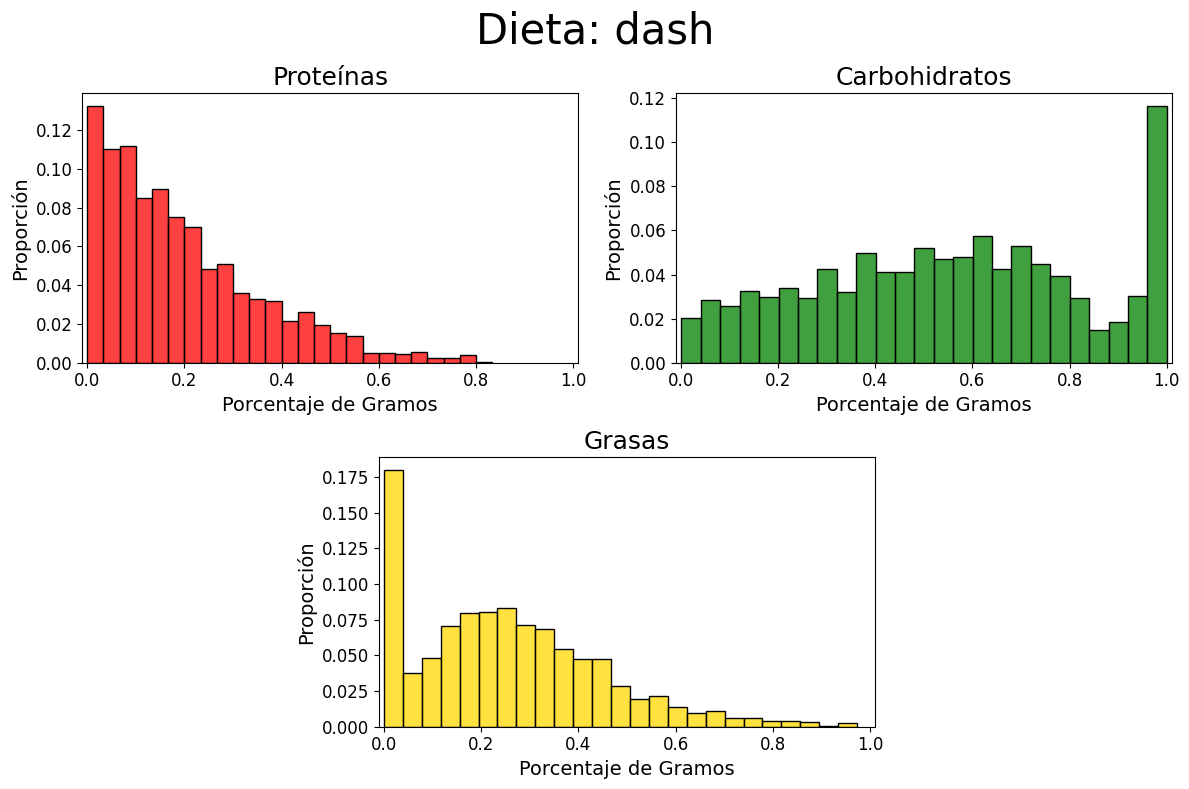
\includegraphics[width=0.85\textwidth]{Resources/2_03_plot_01.png}
            \end{center}

            Como se ha mencionado, el macronutriente relevante para esta dieta son los 
            carbohidratos. Al hacer el contraste entre los diferentes tipos de cocina se 
            puede apreciar un incremente notorio en el primer cuartil de las diferentes 
            cocinas, esto implica qué tan diversificada está esta dieta. En el sentido 
            de que se puede llegar a consumir todo tipo de proporciones sin salirse del 
            marco de la dieta, de otra manera, se podría alcanzar un balance en la ingesta 
            de macronutrientes al considerar recetas de diferentes cocinas.\\

            Debido a que las recetas tienden a tener una alta concentración de carbohidratos 
            se tiene que los otros macronutrientes deben que disiminuir, es decir, bajar 
            su presencia en las recetas; esto se ve reflejado en una correlación negativa. En 
            específico la correlación (negativa) casi perfecta que existe entre carbohidratos y 
            grasas permite explicar que las recetas hacen uso de alimentos bajos en grasas o que 
            disminuyen el consumo de grasas; mientras que las proteínas también disminuye conforme 
            los carbohidratos aumentan pero en una menor medida, esto debido a que se busca disminuir 
            principalmente la ingesta de grasas.

            \begin{center}
                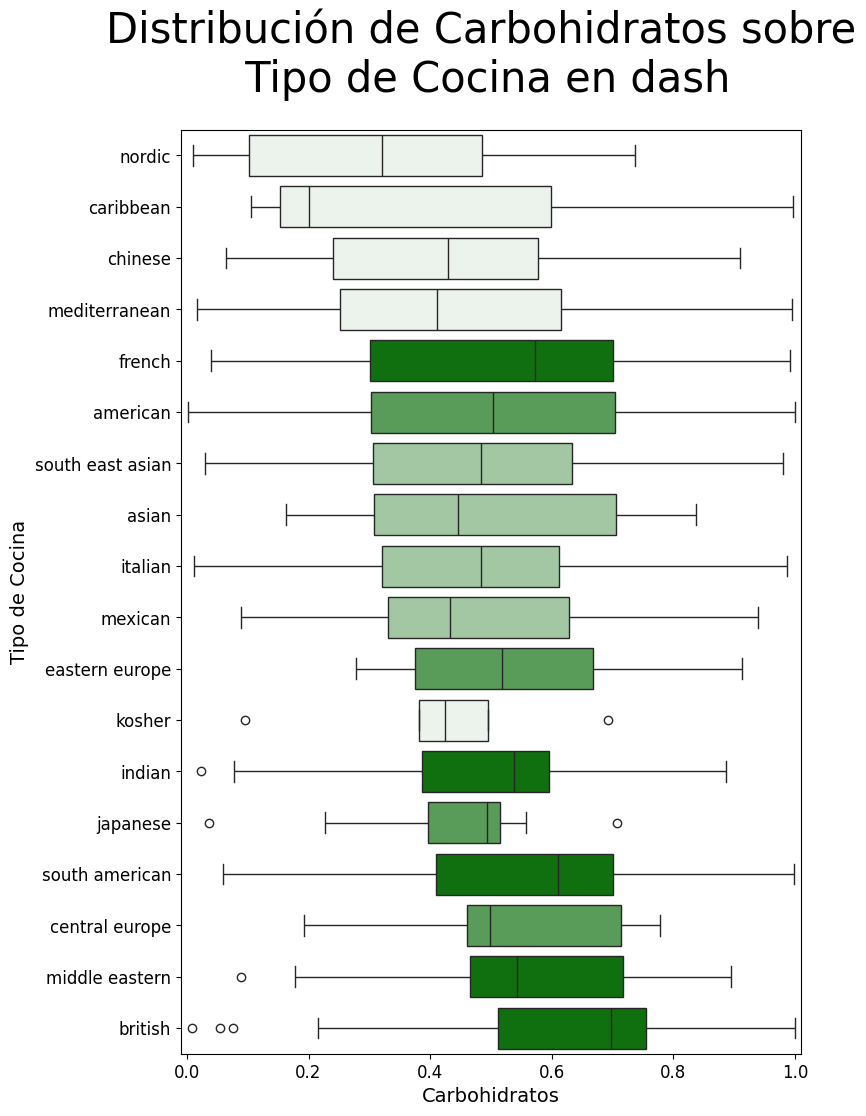
\includegraphics[width=0.65\textwidth]{Resources/2_03_plot_01_1.png}
                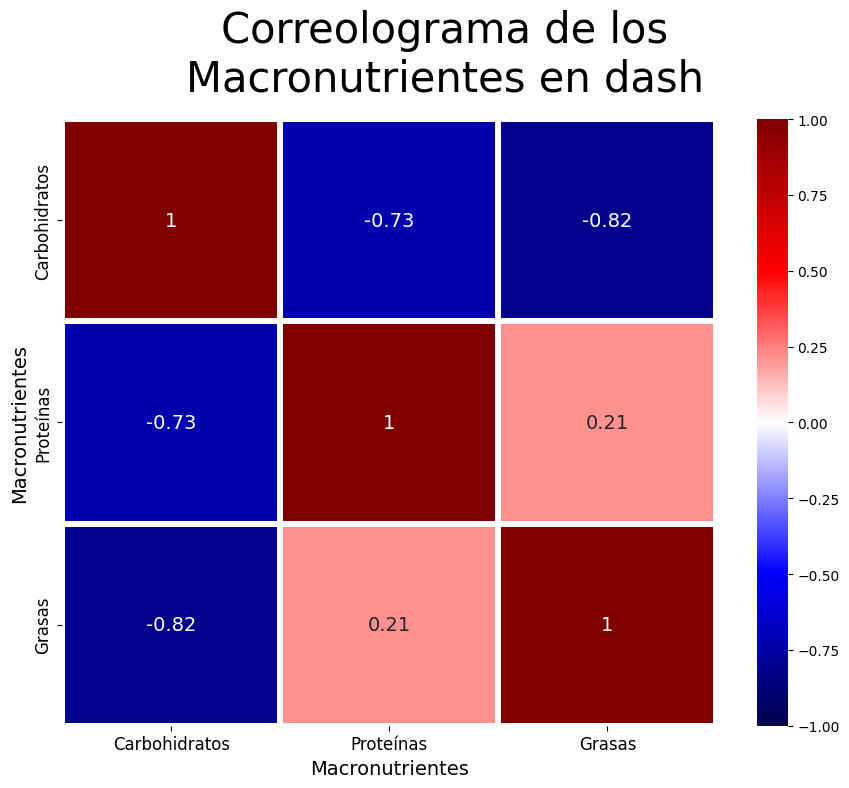
\includegraphics[width=0.6\textwidth]{Resources/2_03_plot_01_4.png}
            \end{center}

        \subsubsection{Dieta Keto}

            Una receta de esta dieta tendrá que, en promedio, el $50\%$ de 
            sus macronutrientes son grasas, esto se relaciona con el hecho de 
            que se intenta inducir la ketosis (principio en que se basa esta         
            dieta); el $30\%$ son proteínas, notando que se intenta reducir 
            el consumo de carbohidratos; y el $20\%$ son carbohidratos, 
            resaltando ser una dieta baja en carbohidratos.\\

            El cincuenta por ciento de las recetas tienen entre el $40\%$ y 
            $60\%$ de grasas en su composición, denotando que existe una alta 
            concentración de recetas con una alta composición en grasas. Y, de 
            igual manera, el cincuenta por ciento de las recetas tienen entre 
            el $8\%$ y $26\%$ de carbohidratos, verificándose el hecho de que 
            se quiere minimizar el consumo de carbohidratos.\\

            En las proteínas, se puede observar que es como un caso intermedio, 
            debido a que, usando su rango intercuartil, la distribución de valores 
            que toma es amplia pero sigue siendo valores menores a los que se puede 
            encontrar en grasas. Esto es consecuencia de que se quiere intentar 
            eliminar el consumo de carbohidratos mientras se incrementa el consumo 
            de grasas.

            \begin{center}
                \begin{tabular}{l|lll}
                    \toprule
                        Medida & Carbs & Protein & Fat \\
                    \midrule
                        Media               & 0.200879 & 0.301777 & 0.497344  \\
                        $Q_1$               & 0.085517 & 0.158284 & 0.405354  \\
                        $Q_2$               & 0.157348 & 0.302900 & 0.505751  \\
                        $Q_3$               & 0.267535 & 0.409453 & 0.591887  \\
                        Desviación Estándar & 0.160609 & 0.167027 & 0.166572  \\
                        Mínimo              & 0.002060 & 0.000000 & 0.000000  \\
                        Máximo              & 1.000000 & 0.856868 & 0.997940  \\
                        Asimetría de Fisher & 1.634945 & 0.314795 & -0.147406 \\
                    \bottomrule
                \end{tabular}
            \end{center}

            Como los tres macronutrientes reportan una desviación estándar similar, 
            se tiene que es indicio de que las recetas son similares en su composición 
            de macronutrientes, es decir, diferentes recetas reportan composiciones 
            semejantes pero que se conforman de distintos alimentos o productos.\\

            Como la proporciones de carbohidratos cuenta con un sesgo positivo, se 
            tiene que refuerza el hecho de ser una dieta baja en carbohidratos. 
            De los aportes de grasas, se observa que su sesgo es despreciable implicando 
            que existen recetas tanto con aportes altos de este macronutriente (lo que se 
            busca) mientras que hay recetas con una contribución baja o nula del mismo.
            
            \begin{center}
                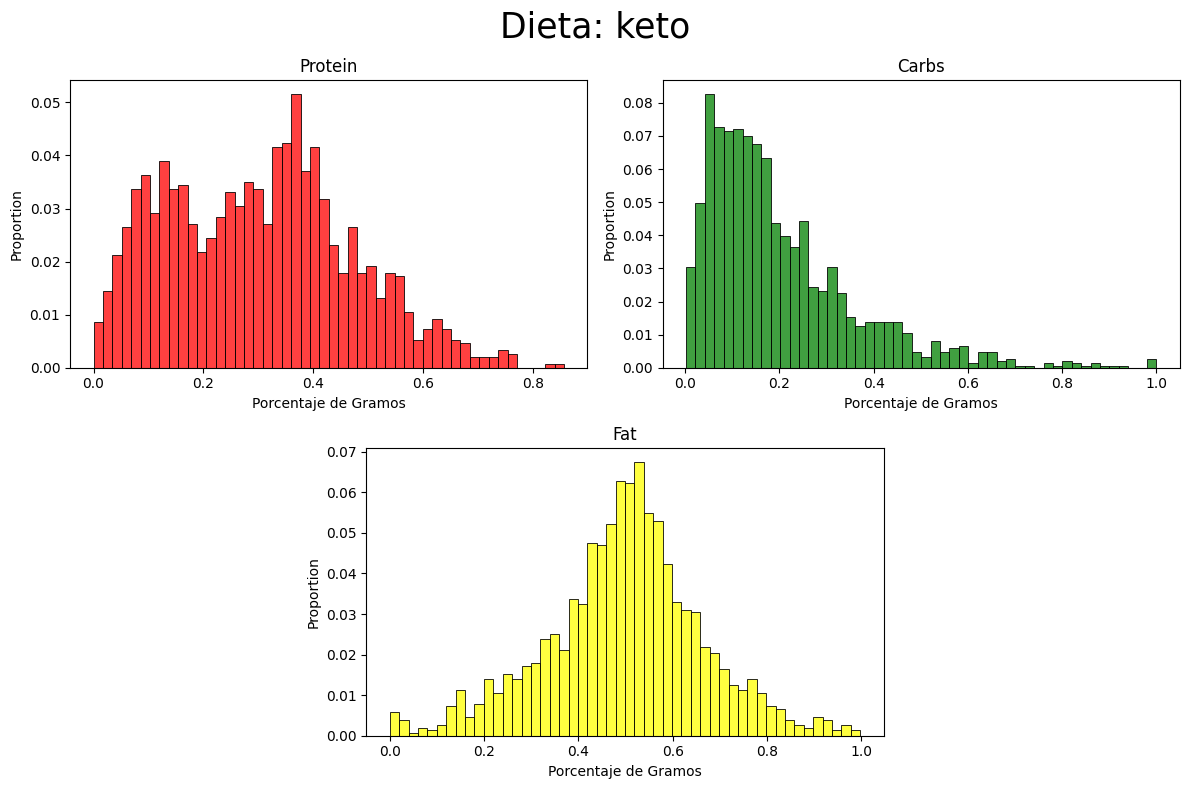
\includegraphics[width=0.85\textwidth]{Resources/2_03_plot_02.png}
            \end{center}

            Para la dieta keto, lo más importante es mantener un consumo alto de grasas, o 
            por al menos mayor que el de carbohidratos. Por lo que al analizar los aportes de grasas 
            en las diferentes cocinas se puede apreciar el como existen países cuyos recetas 
            tienden a tener aportes bajos de grasas, esto es indicativo de que esas recetas no 
            deberían que catalogarse como keto, siendo estas cocinas las de regiones asiáticas
            y América del sur. En cambio, en la mayoría de las demás cocinas sí respetan la 
            tendencia de tener altos aportes en grasas.\\

            Al ser una dieta rica en grasas se espera que la proporción de carbohidratos y proteínas 
            disminuya conforme se incrementa la ingesta de grasas, hecho que se ve reflejado en las 
            correlaciones; por lo que a tener correlaciones negativas permiten explicar la relación 
            de los macronutrientes en esta dieta. También se nota una relación negativa entre carbohidratos y 
            proteínas, esto se relaciona con el hecho de que se quiere disminuir la cantidad de carbohidratos 
            por lo que también se busca incrementar el consumo de proteínas pero sin que sea el macronutriente 
            dominante.

            \begin{center}
                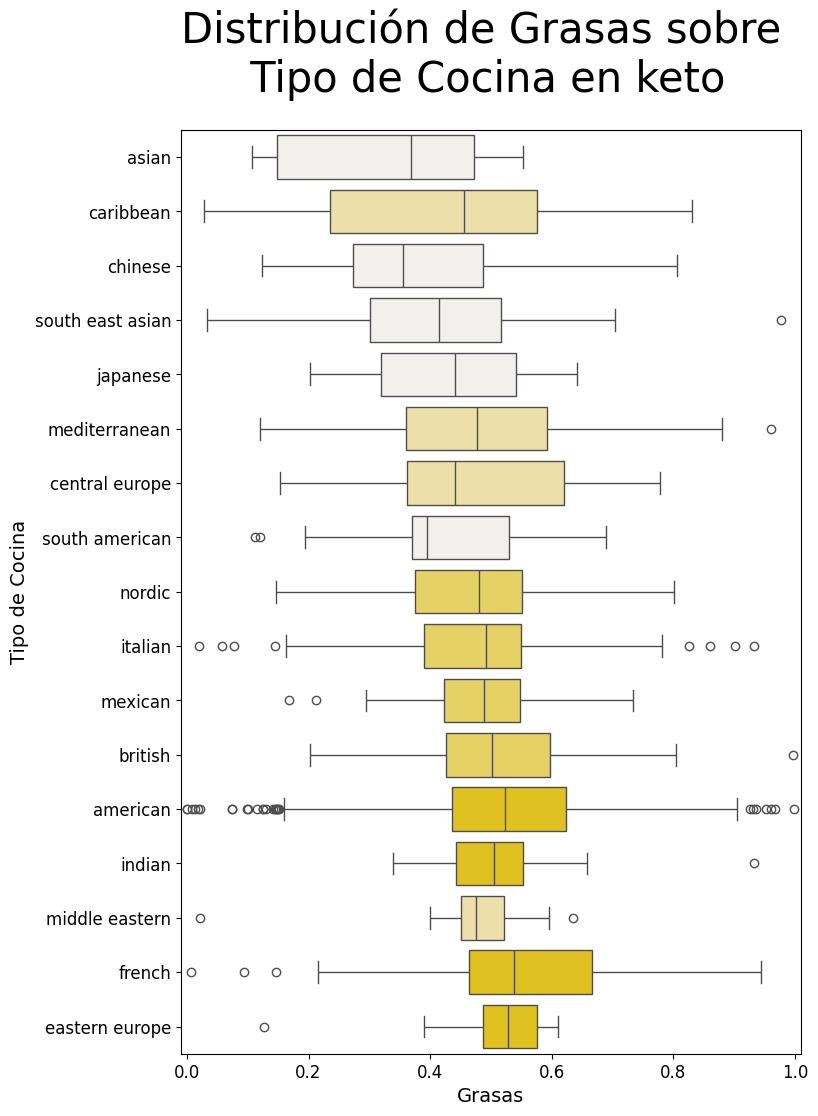
\includegraphics[width=0.65\textwidth]{Resources/2_03_plot_02_3.png}
                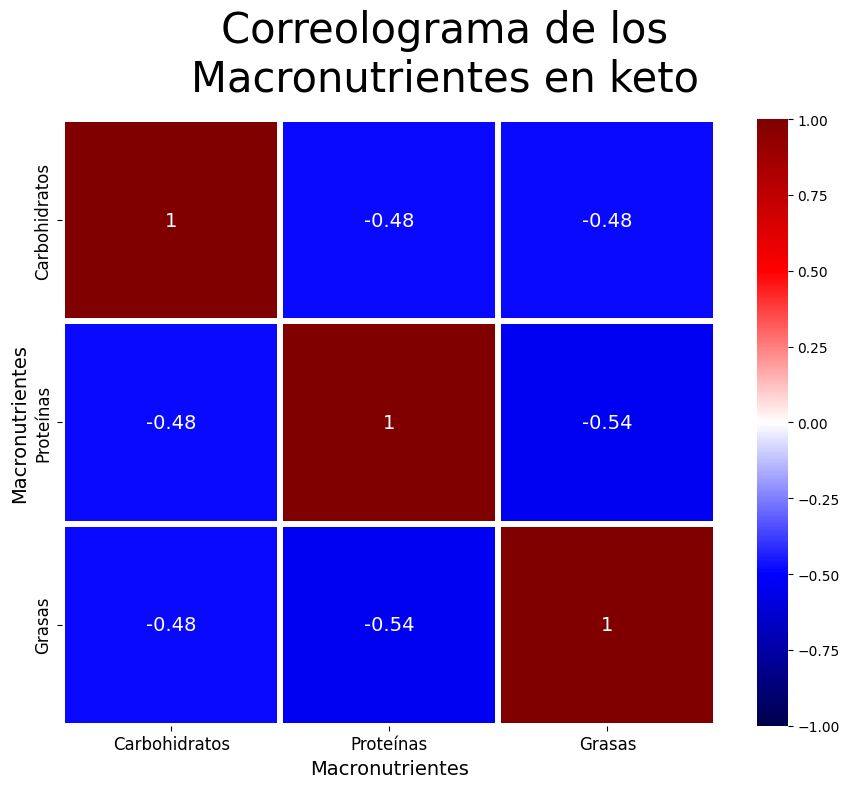
\includegraphics[width=0.6\textwidth]{Resources/2_03_plot_02_4.png}
            \end{center}

        \subsubsection{Dieta Mediterránea}

            Una receta de esta dieta tendrá que, en promedio, el $42\%$ de sus 
            macronutrientes son carbohidratos, esto debido a un alto consumo de 
            productos como, frutas, vegetales y granos enteros; el $30\%$ son 
            grasas, resaltando un alto consumo de nueces y aceite de oliva, como 
            también un consumo moderado de pescado; y el $28\%$ son proteínas, 
            vinculado con un consumo moderado de pescado y aves de corral, y un 
            bajo consumo de carnes rojas.\\

            El cincuenta por ciento de las recetas tienen entre el $25\%$ y $60\%$ 
            de carbohidratos en sus aportes, reflejando una alta variedad de composiciones 
            sobre este macronutriente. Esto debido a los alimentos base de esta dieta y 
            al valor reportada para su desviación estándar,haciendo posible esta 
            diversidad de valores.\\

            En el caso de las proteínas y grasas, muestras distribuciones que siguen 
            patrones similares en el sentido de que sus desviaciones estándar y rangos 
            intercuartiles son similares. Por lo que las recetas, por al menos en estos 
            macronutrientes, tienen composiciones similares. Específicamente, el cincuenta 
            por ciento de ellas tiene entre el $16\%$ y $38\%$ de proteínas	y el $18\%$ y 
            $39\%$ de grasas en la composiciones de estos macronutrientes.

            \begin{center}
                \begin{tabular}{l|lll}
                    \toprule
                        Medida & Carbs & Protein & Fat \\
                    \midrule
                        Media               & 0.424493 & 0.279357 & 0.296150  \\
                        $Q_1$               & 0.249955 & 0.159633 & 0.180357  \\
                        $Q_2$               & 0.439382 & 0.227883 & 0.268336  \\
                        $Q_3$               & 0.607531 & 0.377820 & 0.390404  \\
                        Desviación Estándar & 0.214325 & 0.162853 & 0.160783  \\
                        Mínimo              & 0.006733 & 0.005036 & 0.001731  \\
                        Máximo              & 0.992746 & 0.887557 & 0.968722  \\
                        Asimetría de Fisher & -0.096055 & 0.955922 & 0.869493 \\
                    \bottomrule
                \end{tabular}
            \end{center}

            La amplia variedad en la composición de macronutrientes en las recetas podría 
            estar relacionada con la internacionalización de esta dieta, en específico, de 
            tomar inspiración de recetas y adaptarlas a los productos disponibles en 
            ciertas regiones geográficas.\\

            La proporción de proteínas está segada positivamente y junto con una 
            alta acumulación de recetas con bajo porcentaje de proteínas, se tiene que 
            esta dieta figura como una con bajo consumo de alimentos ricos en proteínas. 
            
            \begin{center}
                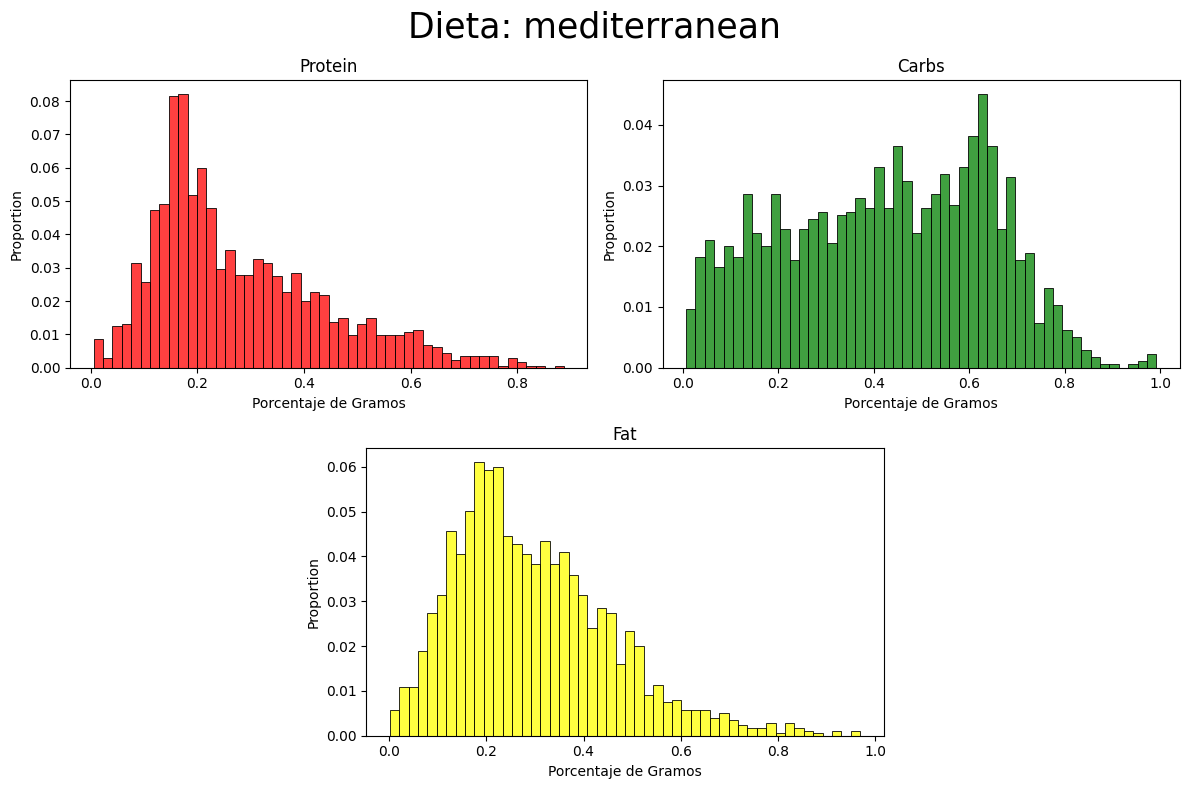
\includegraphics[width=0.85\textwidth]{Resources/2_03_plot_03.png}
            \end{center}

            Debido que para esta receta se cuenta con la región de dónde proviene, la 
            comparativa se vuelve respecto a la distribución de los macronutrientes en 
            la cocina del mediterráneo. Del análisis e histogramas, donde más podría haber 
            diferencias es en las grasas debido a su desviación estándar y rango de valores. 
            Al hacer la comparativa se puede observar que conforme las regiones a las que 
            pertenecen las cocinas se alejan más del mediterráneo crece más las discrepancia, 
            ya sea por un cambio total en la distribución o por una traslación ligera en los 
            cuartiles.\\

            Al ser una dieta rica en carbohidratos se tiene que conforme la presencia de 
            este macronutriente se incrementa, los otros macronutrientes disminuyen en 
            una relación casi lineal, es decir, se tiene una alta concentración de carbohidratos. 
            Mientras que las proteínas y grasas tienden a no tener una relación lineal, indicando 
            que las recetas no siguen una preferencia sobre estos macronutrientes al momento de 
            que se determinan los aportes de los mismos, es decir, es igual de probable ver 
            recetas que tienen las composiciones de proteínas y grasas invertidas.

            \begin{center}
                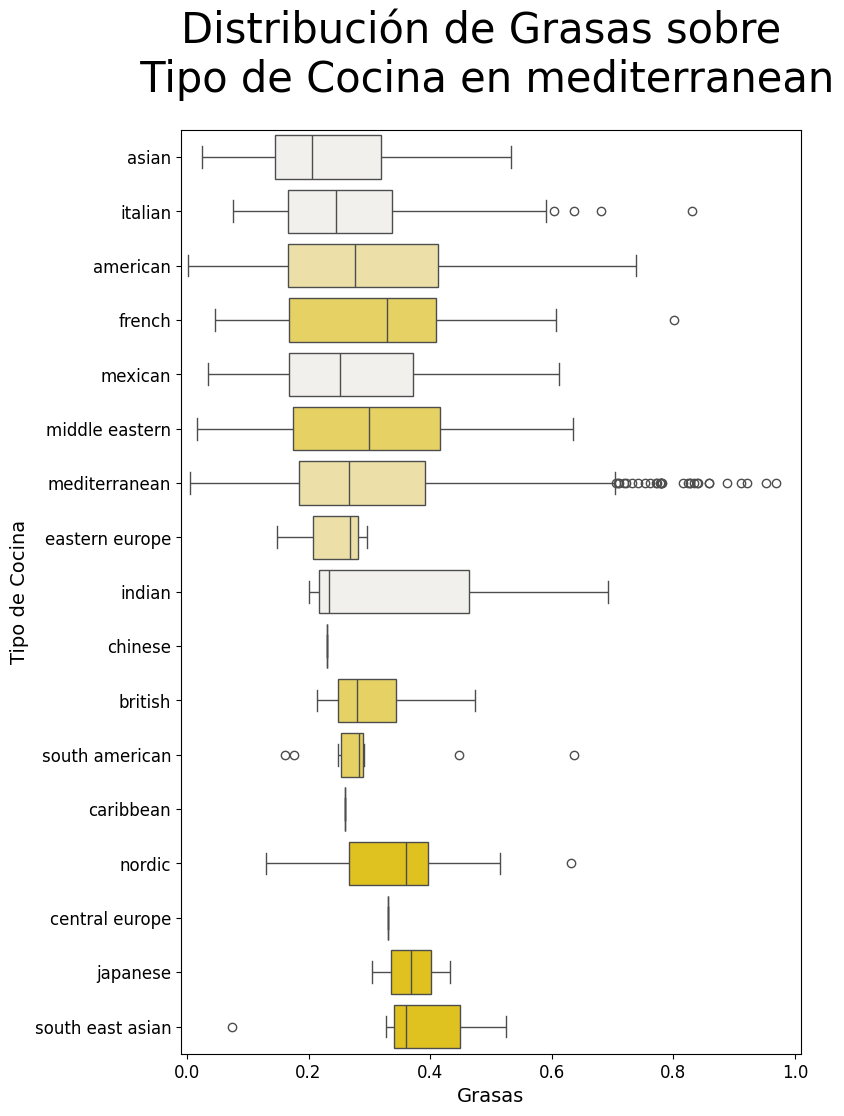
\includegraphics[width=0.65\textwidth]{Resources/2_03_plot_03_3.png}
                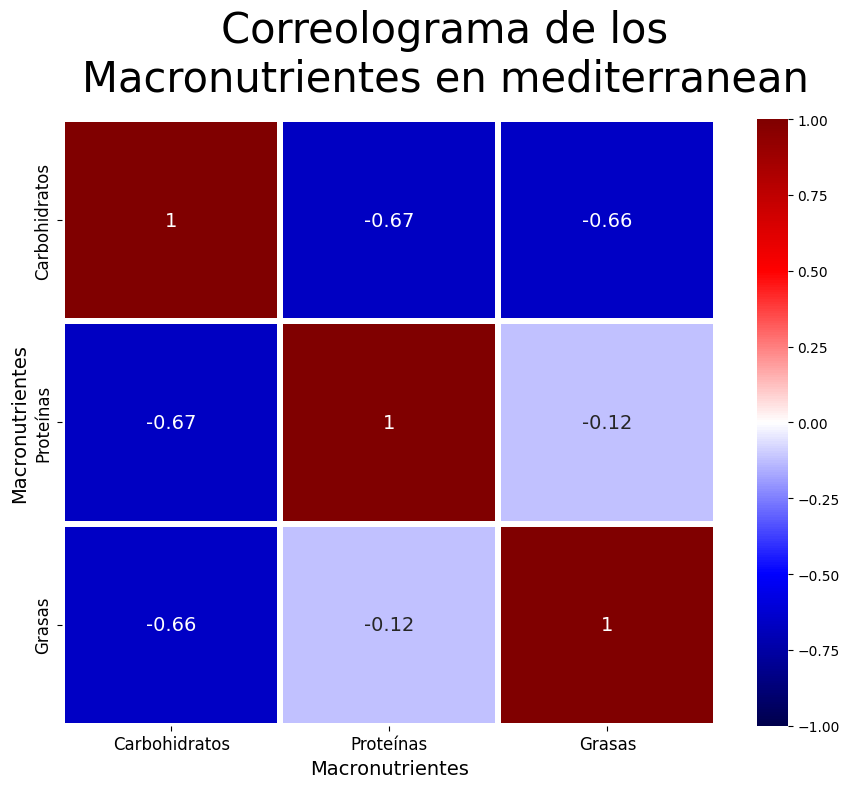
\includegraphics[width=0.6\textwidth]{Resources/2_03_plot_03_4.png}
            \end{center}

        \subsubsection{Dieta Paleo}

            Una receta de esta dieta tendrá que, en promedio, el $38\%$ de sus 
            macronutrientes son grasas y el $37\%$ son carbohidratos, esto se 
            relaciona con el consumo de productos como frutas, vegetales, nueces 
            y semillas; y el $25\%$ son proteínas cuyas principales fuentes son 
            carnes margas y pescado.\\

            El cincuenta por ciento de las recetas tienen entre el $19\%$ y $51\%$ 
            de carbohidratos en sus aportes, indicando una alta variedad de recetas 
            respecto a este macronutriente, esto se debe al consumo de alimentos que 
            se encuentran en la naturaleza o en estado salvaje (excluyendo algunos 
            de ellos).\\

            Como las proteínas y grasas tienen desviaciones estándar similares, refleja 
            que los alimentos y productos asociados a estos macronutrientes no tengan 
            una alta diversidad. Es decir, las recetas tienen muchos productos y alimentos 
            en común. En cambio, sus rangos intercuartiles difieren, mostrando como 
            las proteínas, sus valores, están más concentradas en un rango menor en 
            comparación con el de las grasas.

            \begin{center}
                \begin{tabular}{l|lll}
                    \toprule
                        Medida & Carbs & Protein & Fat \\
                    \midrule
                        Media               & 0.371307 & 0.249693 & 0.379000  \\
                        $Q_1$               & 0.192399 & 0.102963 & 0.256579  \\
                        $Q_2$               & 0.351300 & 0.205532 & 0.382447  \\
                        $Q_3$               & 0.515054 & 0.375392 & 0.488116  \\
                        Desviación Estándar & 0.221506 & 0.175031 & 0.175471  \\
                        Mínimo              & 0.003612 & 0.000000 & 0.001404  \\
                        Máximo              & 0.987368 & 0.858503 & 0.968835  \\
                        Asimetría de Fisher & 0.488656 & 0.711408 & 0.312673  \\
                    \bottomrule
                \end{tabular}
            \end{center}

            La posible limitante de alimentos asociados a proteínas	y grasas 
            podría impactar en que las recetas estén hechas con los mismos productos 
            dentro de la misma región geográfica. Estos se relacionaría con una 
            baja variedad en la presencia de estos macronutrientes.\\

            Se observa como las recetas tienden a tener una contribución moderada de 
            carbohidratos y grasas, esto se relaciona con los principales alimentos 
            que son consumidos en esta dieta. Mientras que sus aportes de proteínas 
            son bajas en comparación con los otros dos macronutrientes.
            
            \begin{center}
                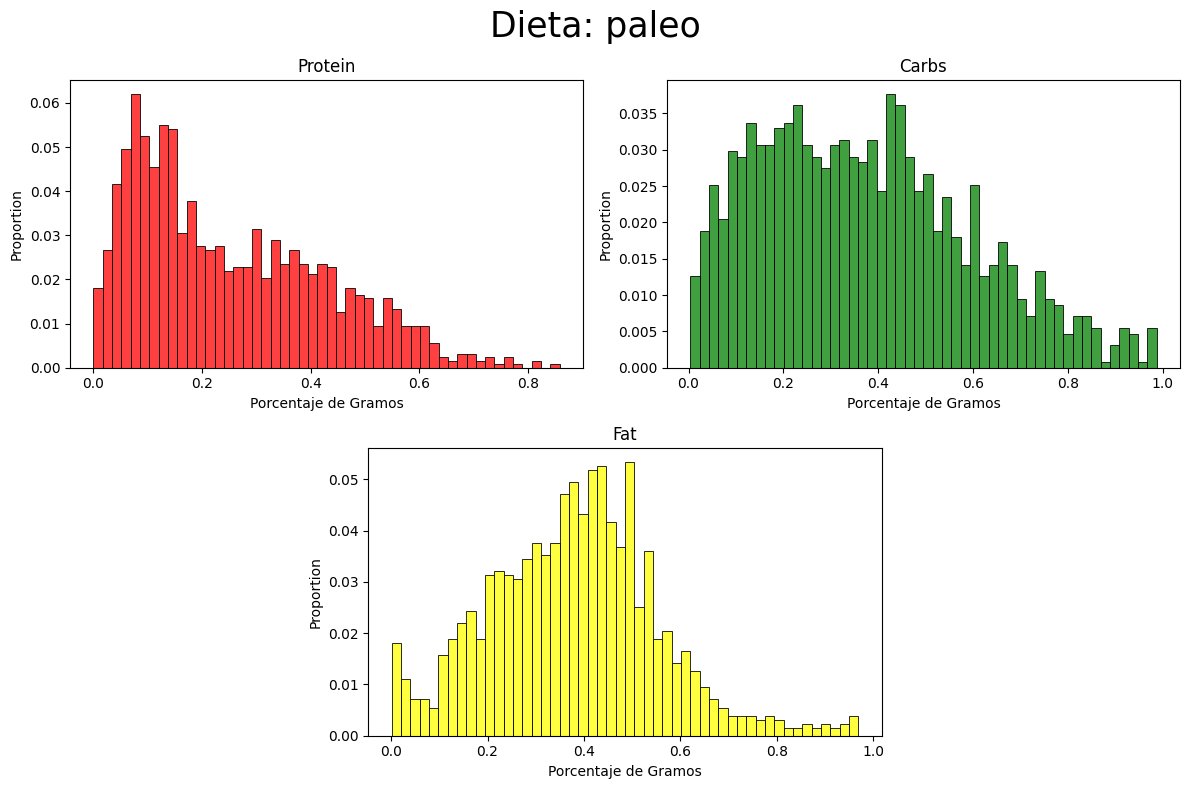
\includegraphics[width=0.85\textwidth]{Resources/2_03_plot_04.png}
            \end{center}

            Como las proteínas es un macronutriente que tiende a tener una presencia 
            baja en las recetas, como se mencionó, podría deberse por las regiones geográficas. 
            Las regiones en donde más se aprovecharon de los recursos hídricos tienden a tener 
            una ingesta alta de proteínas, esto relacionado al consumo de alimentos provenientes 
            del mar. Mientras que regiones sin tantas salidas al mar y cercanas a las ciudades 
            primitivas tienden a tener aportes de proteínas	menores.\\

            Debido a que los principales alimentos disponibles en la naturaleza son los de 
            origen vegetal, ricos en carbohidratos, se tiene que al tener una correlación de 
            igual valor en los otros dos macronutrientes muestra como posiblemente la disponibilidad 
            de alimentos ricos en proteínas y grasas se encuentren en el mismo nivel, es decir, 
            el encontrar un alimento rico en proteínas se vuelve equivalente a encontrar uno rico 
            en grasas. Esto se ve reforzado al ver su correlación, que es una débil, mostrando que 
            posiblemente muchas de las recetas tengan composiciones en proteínas y grasas en ordenes 
            invertidos.

            \begin{center}
                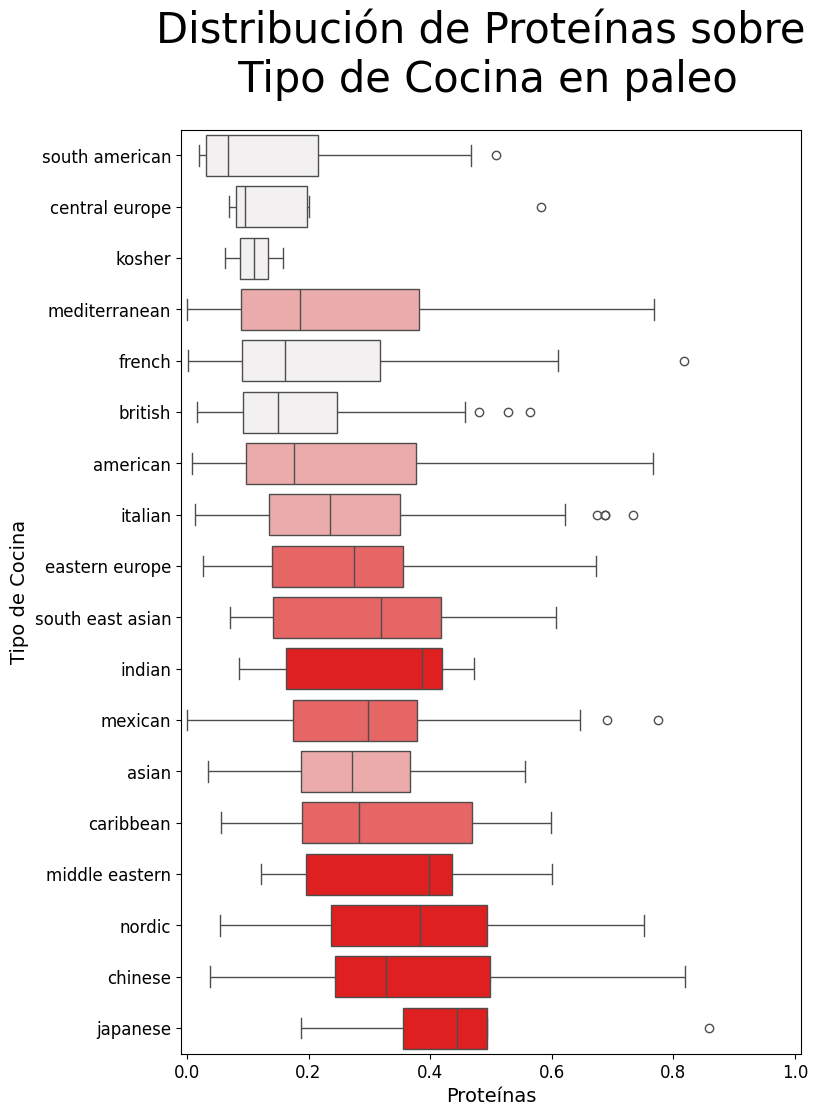
\includegraphics[width=0.65\textwidth]{Resources/2_03_plot_04_2.png}
                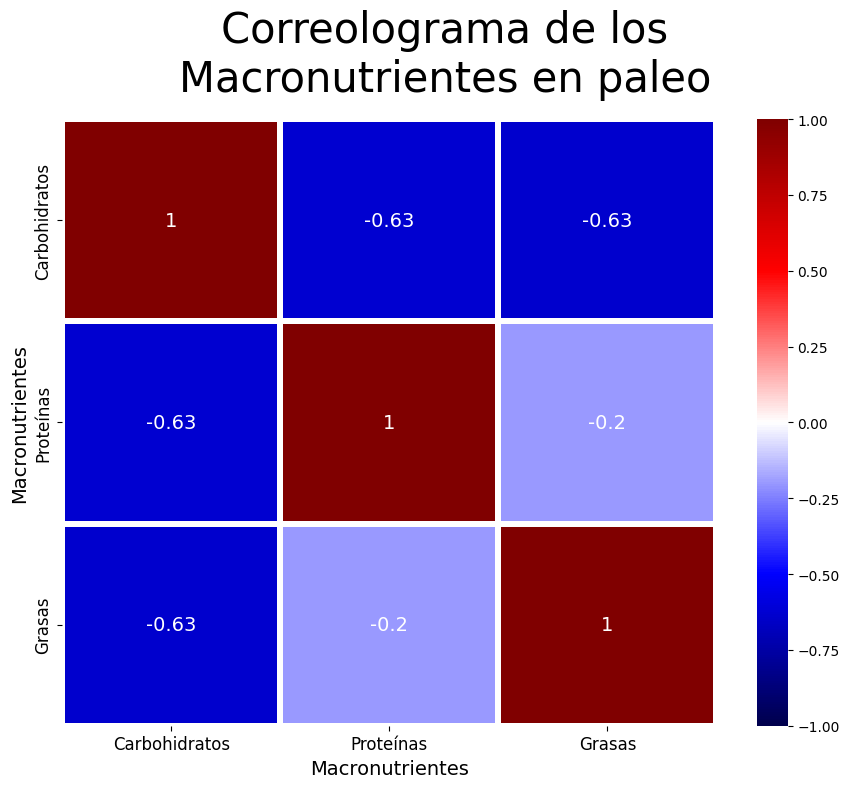
\includegraphics[width=0.6\textwidth]{Resources/2_03_plot_04_4.png}
            \end{center}

        \subsubsection{Dieta Vegana}

            Una receta de esta dieta tendrá que, en promedio, el $60\%$ de 
            sus macronutrientes son carbohidratos, que provienen de fuentes 
            como vegetales, frutas, cereales y legumbres; el $25\%$ son grasas, 
            relacionadas con el consumo de nueces y semillas; y el $15\%$ son 
            proteínas, esto debido a un nulo consumo de alimentos de origen 
            animal y que estas fuentes son reemplazadas por fuentes vegetales.\\

            El cincuenta por ciento de las recetas tienen entre el $50\%$ y el $71\%$ 
            de carbohidratos en su composición, esto debido al alto consumo de 
            alimentos ricos en carbohidratos en origen vegetal, los cuales son 
            muy diversos.\\

            Mientras que el cincuenta por ciento de las recetas tienen entre el $14\%$ y 
            el $34\%$ de grasas en su composición, esto se relaciona al hecho de que 
            existen alimentos de origen vegetal ricos en grasas no animales.\\
            
            En las proteínas, se puede observar un rango intercuartil reducido y una 
            desviación estándar reducida, esto evoca a que las recetas tengan bajos 
            aportes de proteínas así como también los valores de aportes se concentren 
            en un rango reducido. En específico, el cincuenta por ciento de las recetas 
            tienen entre el $8\%$ y el $19\%$ de proteínas.

            \begin{center}
                \begin{tabular}{l|lll}
                    \hline
                        Medida & Carbs & Protein & Fat \\
                    \hline
                        Media               & 0.593968 & 0.148489 & 0.257543  \\
                        $Q_1$               & 0.504070 & 0.085339 & 0.142575  \\
                        $Q_2$               & 0.626246 & 0.139688 & 0.231518  \\
                        $Q_3$               & 0.714679 & 0.190381 & 0.344529  \\
                        Desviación Estándar & 0.171203 & 0.086088 & 0.160277  \\
                        Mínimo              & 0.000330 & 0.001921 & 0.000112  \\
                        Máximo              & 0.986872 & 0.647416 & 0.994887  \\
                        Asimetría de Fisher & 0.189556 & 0.922401 & 0.461455  \\
                    \hline
                \end{tabular}
            \end{center}

            Debido a que los carbohidratos y grasas reportan desviaciones estándar 
            similares, sería indicio de que las recetas tienen composiciones similares 
            para estos dos macronutrientes.\\

            De las proporciones de proteínas, se resalta una alta acumulación de 
            recetas con bajos aportes de proteínas, esto hace de esta dieta una 
            con bajo consumo de proteínas. Lo último debido a que las principales 
            fuentes proteínas son animales y haciendo que los aportes de carbohidratos 
            sean altos en comparación con los otros dos macronutrientes.

            \begin{center}
                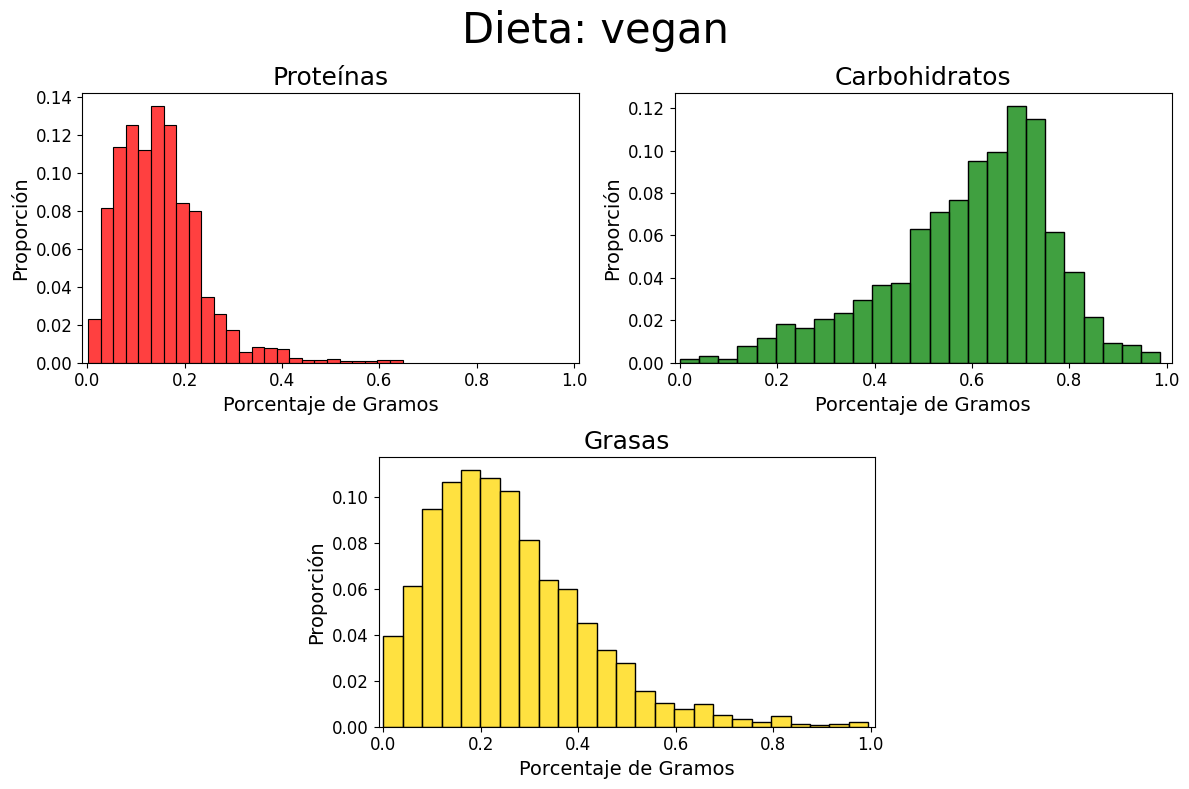
\includegraphics[width=0.85\textwidth]{Resources/2_03_plot_05.png}
            \end{center}

            Debido a que las proteínas es el macronutriente que menor presencia tiene 
            en esta dieta, se tiene que se vuelve relevante para el contraste entre regiones. 
            Se puede observar como en la mayoría de los países tienen distribuciones donde 
            las proteínas toma valores bajos, que es el patrón esperado, pero en cambio 
            existen otros donde puede tomar valores un poco más altos y con una probabilidad 
            también alta.\\

            Debido a ser una dieta con bajo consumo de proteínas e incluso limitadas, se tiene 
            que se pueden ver como si fuera un valor fijo, haciendo que los carbohidratos y 
            grasas sean los únicos macronutrientes que pueden variar en la composición de una 
            receta, esto se ve reflejado al ver como están en una correlación perfecta por lo 
            que las recetas tienen una mayor diversidad (valores que pueden tomar) sobre estos 
            macronutrientes.

            \begin{center}
                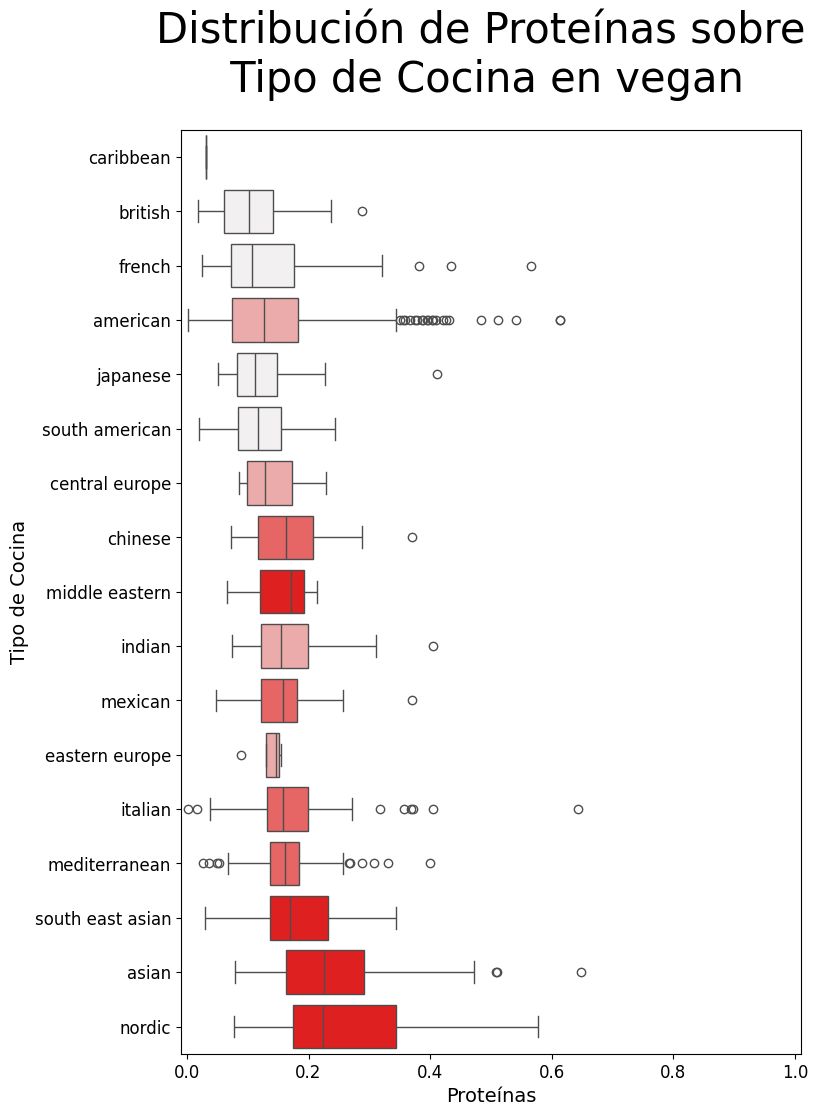
\includegraphics[width=0.65\textwidth]{Resources/2_03_plot_05_2.png}
                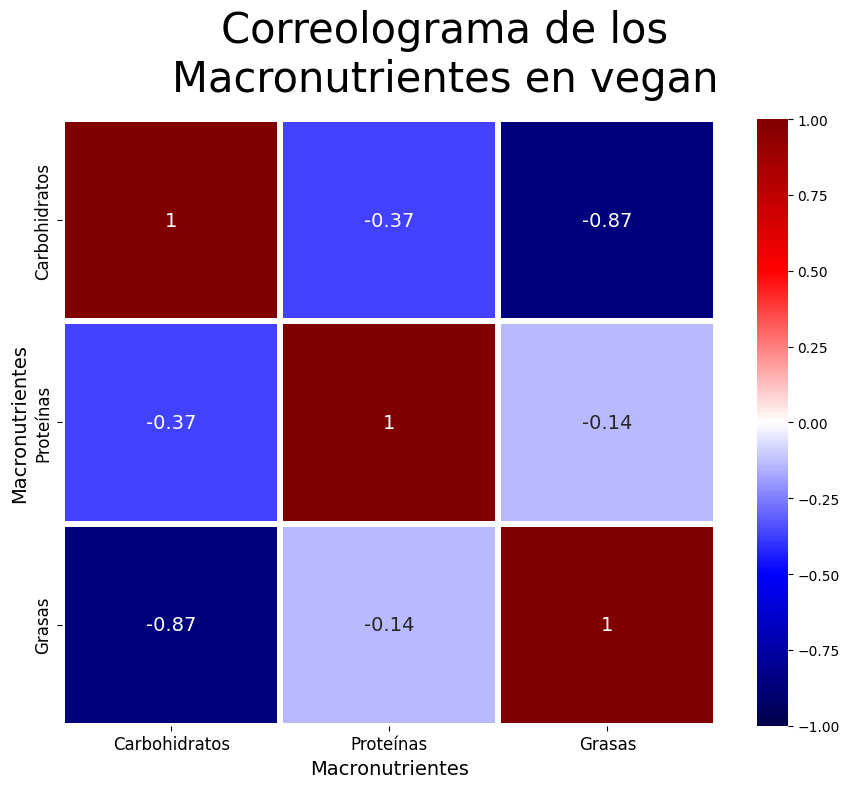
\includegraphics[width=0.6\textwidth]{Resources/2_03_plot_05_4.png}
            \end{center}

        \subsubsection{Gráfico de Cajas y Bigotes de la distribución de Macronutrientes por Dieta}
            Se anexan las gráficas de cajas y bigotes de las distribuciones de los 
            macronutrientes por dieta para apoyar las observaciones realizadas anteriormente. 
            Resaltando el comportamiento esperado en los macronutrientes por dieta que, junto 
            con el análisis dan paso a las reglas que se aplicarán para la eliminación de recetas 
            atípicas que presentan las diferentes dietas.

            \begin{center}
                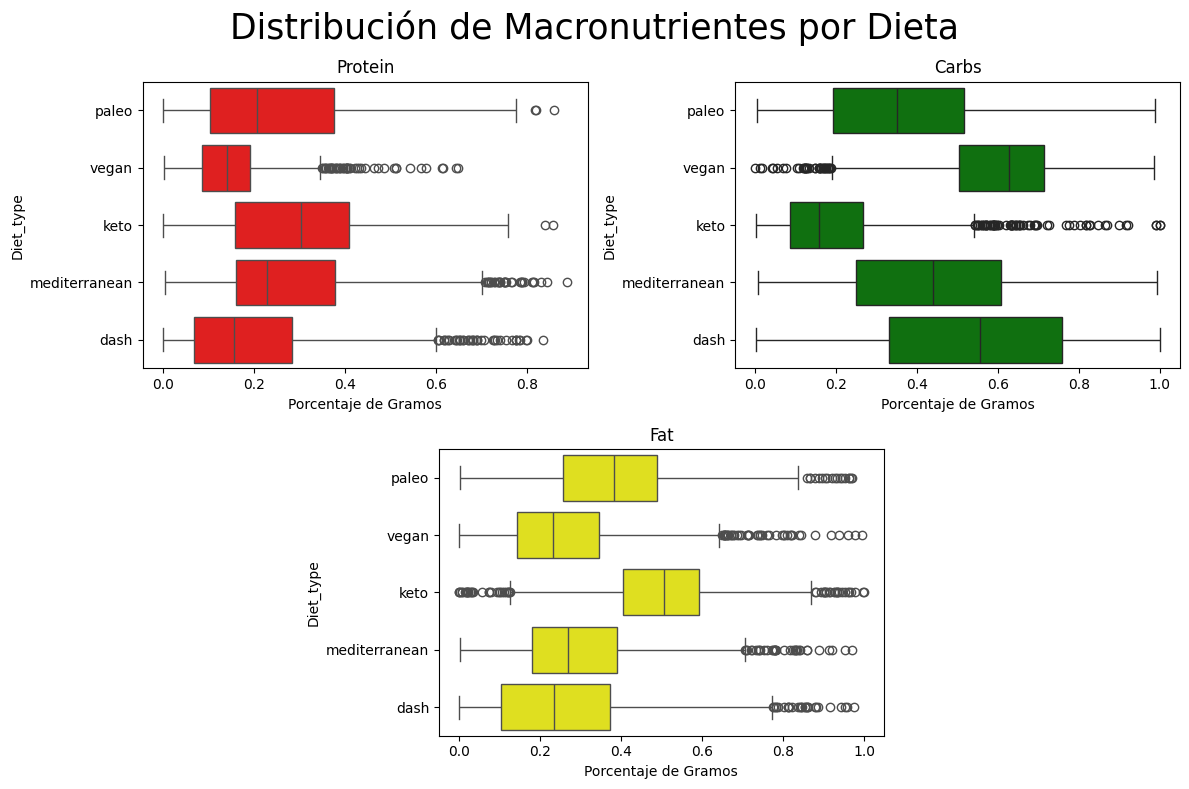
\includegraphics[width=0.95\textwidth]{Resources/2_03_plot_06.png}
            \end{center}
    
    \subsection{Caracterización de las Distribuciones de los Macronutrientes}
        Para lograr una caracterización de las distribuciones de los macronutrientes 
        en cada una de las dietas, se vuelve necesario el reconocer que las distribuciones 
        pertenecen a la familia de las distribuciones beta; esto debido al rango de valores 
        que pueden tomar, el soporte de la distribución, es $[0,1]$. La familia de distribuciones 
        beta son de la forma\cite{beta_distribution}:

        $$F(x;\alpha,\beta) = \frac {x^{\alpha -1}(1-x)^{\beta -1}}{\mathrm {B} (\alpha ,\beta )}$$ 

        Lo que se realiza es el ajuste de una distribución de esta familia y se realiza 
        un Q-Q plot entre la distribución ajustada (teórica) y de la distribución empírica 
        o muestral de los datos. Donde se muestran los parámetros de la distribución, es 
        decir, los valores $\alpha$ y $\beta$ que caracteriza cada una las mismas.\\

        \begin{center}
            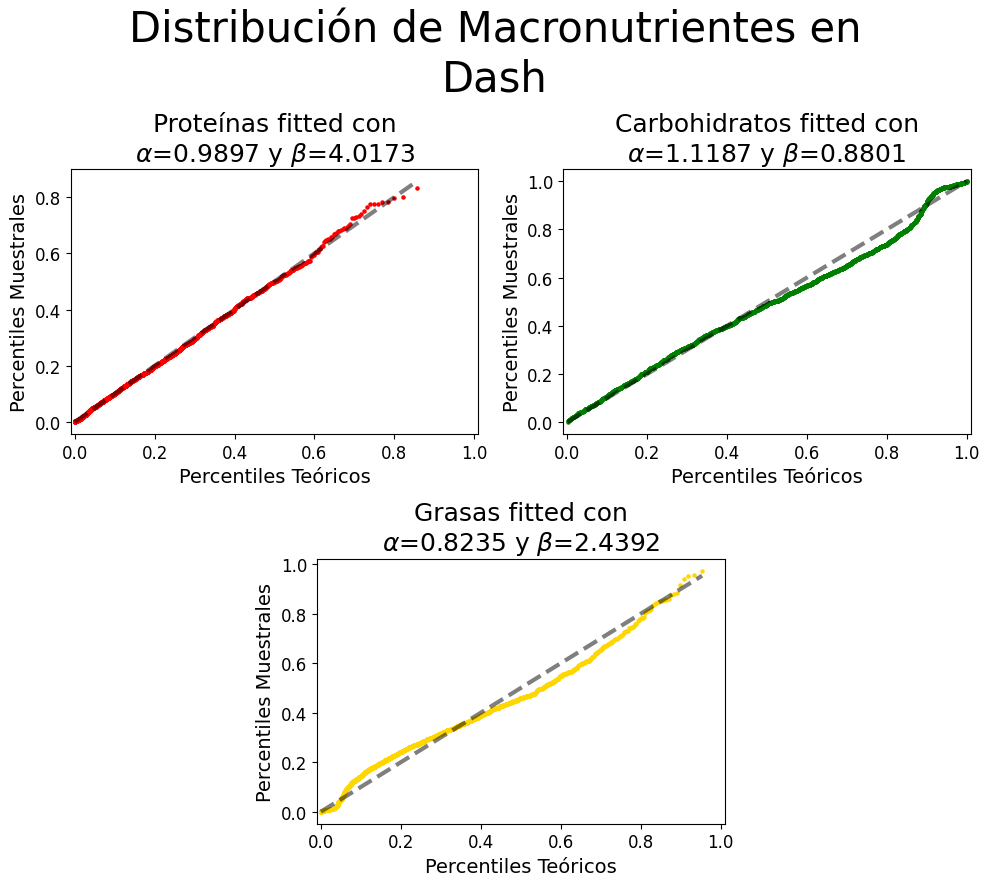
\includegraphics[width=0.8\textwidth]{Resources/5_05_plot_1.png}
            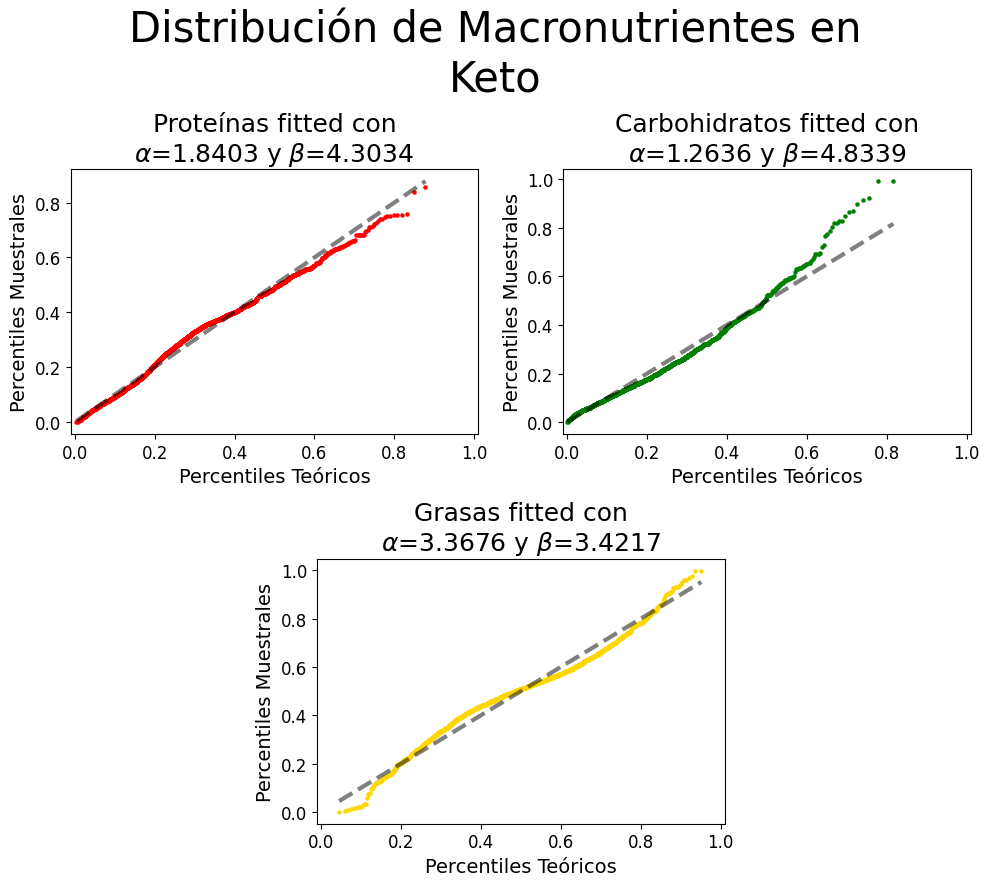
\includegraphics[width=0.8\textwidth]{Resources/5_05_plot_2.png}
            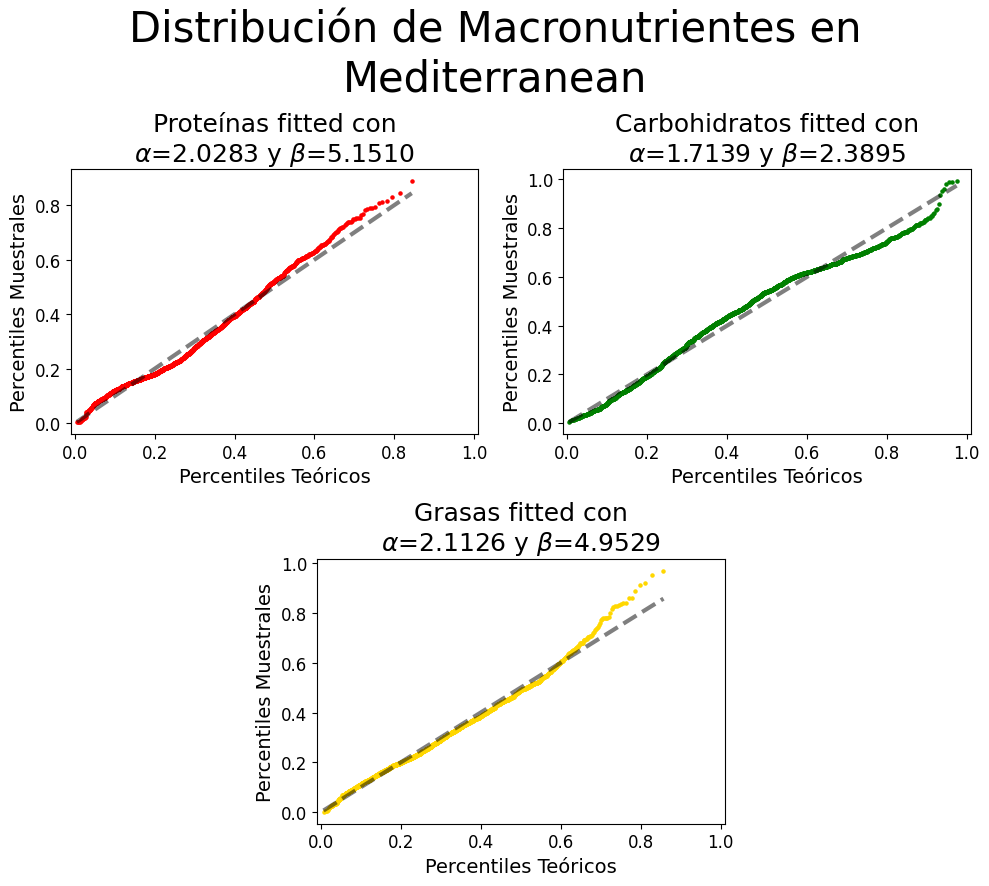
\includegraphics[width=0.8\textwidth]{Resources/5_05_plot_3.png}
            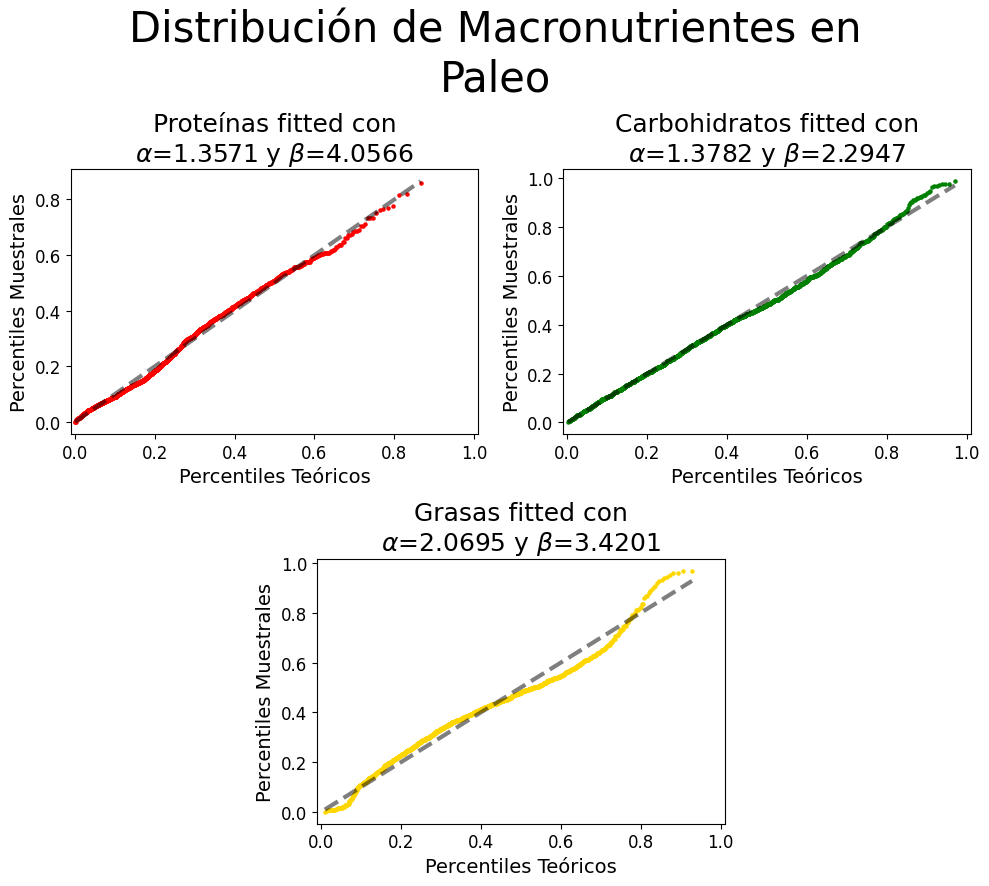
\includegraphics[width=0.8\textwidth]{Resources/5_05_plot_4.png}
            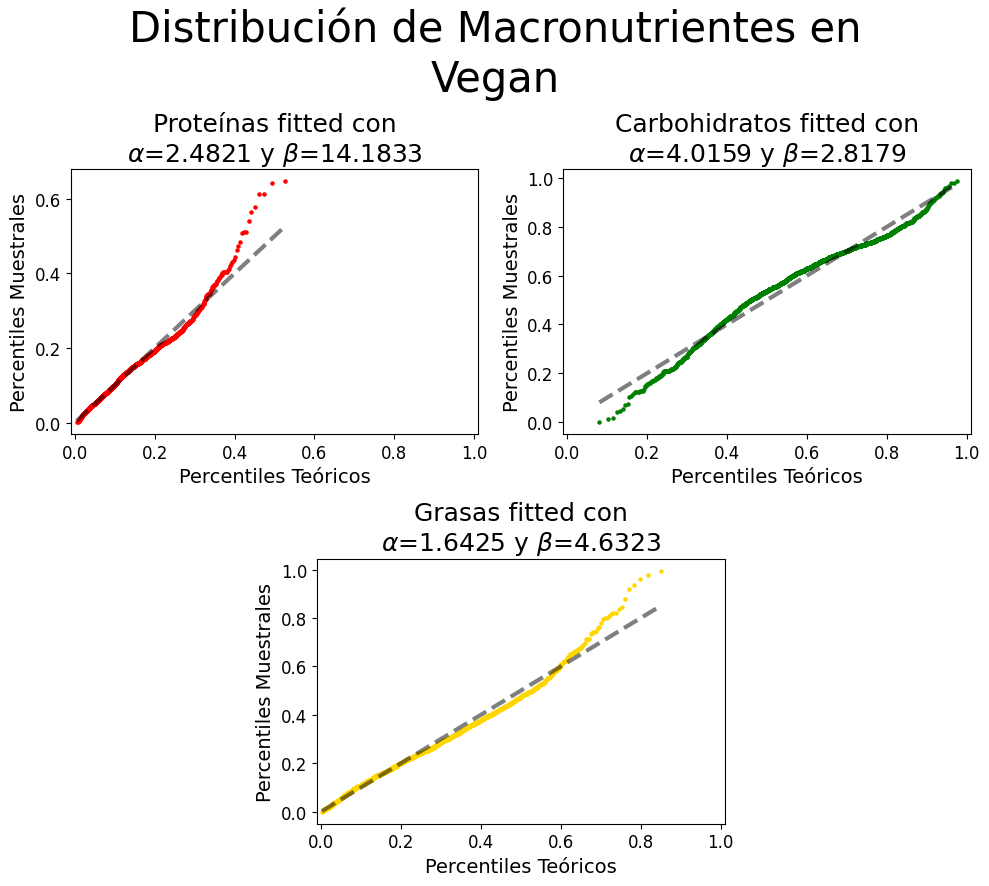
\includegraphics[width=0.8\textwidth]{Resources/5_05_plot_5.png}
        \end{center}

        En los diferentes Q-Q Plots se puede apreciar el como los percentiles se alejan 
        de la recta identidad, esto se debe a la presencia de outliers que modifican 
        el comportamiento de la propia distribución, evocando una tendencia diferente a 
        la de una recta. Por ello, se vuelve necesario un tratamiento sobre los valores 
        atípicos, debido a que en las regiones en donde se consideran valores normales, 
        según los box plots, sí siguen la tendencia de la recta, o de los valores teóricos.\\

        Debido la cantidad de instancias con las que se cuentan por dieta, se tiene que 
        los resultados de las distribuciones ajustadas para cada macronutriente y dieta 
        son confiables, por lo tanto, se puede concluir que éstas son diferentes entre sí, 
        o por al menos lo suficiente para mostrar que cada dieta sigue diferentes patrones 
        en la ingesta de macronutrientes.

\newpage

\section{Pruebas de Hipótesis Por Dieta}

    Para cada una de las pruebas se hace uso de una significancia de $\alpha = 0.05$, 
    para las diferentes pruebas se reportan los p valores (p-value) y el valor del 
    estadístico que se obtuvieron, en los casos que sea posible. El procedimiento 
    desarrollado en esta sección se encuentra en la sección de mismo nombre y 
    enumeración en la libreta de Jupyter que se puede encontrar en \href{https://github.com/alexisuaguilaru/Analysis_Nutritional_Information/blob/main/Documentation/AlexisAguilar_Reporte.ipynb}{Analysis Nutritional Information} 
    donde se expone el código y resultados más en ``crudo'' (sin interpretación).

    \subsection{Dieta DASH}
        \textbf{Preámbulo}\\
        { 
            Se tiene el objetivo de probar si esta dieta se encuentra 
            en balance nutricional, es decir, si se llega a consumir la 
            misma proporción de macronutrientes diariamente. 
            Se realiza el supuesto de que en un día normal se consumen 
            cinco comidas, el equivalente a cinco recetas, por lo que 
            muestreando 50 días siguiendo esta dieta bastaría 
            para probar de manera significativa si la dieta DASH está en 
            balance nutricional. 
            Para generar el muestreo de 50 días se vuelve equivalente a 
            que se muestrean de forma aleatoria 250 recetas que forman 
            grupos de 5 recetas para después determinar las proporciones 
            de macronutrientes que son consumidos al consumir los macronutrientes 
            de estas recetas.\\
        }

        \textbf{Prueba de Hipótesis}\\ 
        {
            Con las muestras de las proporciones de macronutrientes se realiza 
            un conjunto de hipótesis por cada macronutriente, teniendo lo 
            siguiente:

            \begin{align*}
                H_0 :& \overline{x}_M = 1/3  \\
                H_1 :& \overline{x}_M \ne 1/3 
            \end{align*}
        
            Donde $M$ se refiere a uno de los tres macronutrientes con los que 
            se cuenta. El signo de $\ne$ indica que la prueba será de dos colas 
            debido a que se quiere capturar cualquier diferencia significativa 
            por muy mínimo que sea. Y como el tamaño de la muestra es lo suficientemente 
            grande, se puede suponer que la distribución de la media muestral es 
            normal, por lo tanto la prueba que se va usar es la Prueba t para obtener 
            resultados más robustos.\\
        }

        \textbf{Discusión de Resultados}\\
        {
            Se tienen los siguientes resultados de las pruebas:

            \begin{center}    
                \begin{tabular}{lrr}
                    \toprule
                        \textbf{Macronutriente} & \textbf{Valor P} & \makecell{\textbf{Estadístico}\\\textbf{Calculado t}} \\
                    \midrule
                        \emph{Carbohidratos} & 2.4193e-12 &   9.2605 \\
                        \emph{Proteínas}     & 5.0144e-14 & -10.4219 \\
                        \emph{Grasas}        & 0.003801   &  -3.0389 \\
                    \bottomrule
                \end{tabular}
            \end{center}

            Debido al umbral de significancia $\alpha$, se tiene que ninguno 
            de los tres macronutrientes se encuentra en balance nutricional. 
            Lo anterior implica que la dieta DASH, declarada como una dieta 
            saludable para la condición cardiovascular, no verifica estar en 
            balance, esto representa que los alimentos, por lo tanto las recetas, 
            favorecen el consumo de ciertos grupos alimentarios sobre otros. 
            Esto se ve reflejado al ver como el valor del estadístico en 
            carbohidratos reporta ser el más alto, indicando que puede deberse 
            a un alto consumo de alimentos de origen vegetal que, además, pueden 
            ser ricos en otros micronutrientes esenciales para controlar la 
            hipertensión y la salud cardiovascular. Mientras que el consumo de 
            proteínas y de grasas se ve penalizado, por tener signos negativos, 
            esto es indicativo de que en la dieta DASH los alimentos provenientes de 
            estos macronutrientes tienen un mayor control y regularización sobre 
            las cantidades que son consumidas.
        }

    \subsection{Dieta Keto}
        \textbf{Preámbulo}\\
        {
            Se tiene el objetivo de probar si en todas las cocinas de esta dieta 
            se verifica que el consumo de carbohidratos es menor al de grasas, 
            refiriéndose al principio de la dieta keto. Debido a que alguna de las cocinas no cuentan 
            con suficientes instancias de recetas se tiene que esta prueba se 
            divide en dos casos y, por lo tanto, dos tipos de pruebas.\\
        }

        \textbf{Prueba de Hipótesis}\\
        {
            Como se mencionó, sin importar el tipo de caso, el conjunto de hipótesis 
            son de la forma:
            
            \begin{align*}
                H_0 : \overline{c}_C = \overline{f}_C \\
                H_1 : \overline{c}_C < \overline{f}_C
            \end{align*}

            Donde $\overline{c}_C$ y $\overline{f}_C$ representan, según sea el caso, 
            la media o la mediana de los carbohidratos y grasas, respectivamente, de 
            una cocina $C$. 
            Los casos se dividen según lo siguiente: Si la cantidad de recetas es menor 
            o igual a $30$, entonces se hace uso de la Prueba de Rangos de Wilcoxon; en 
            caso contrario se realiza la Prueba t junto con la Prueba de Levenne para 
            probar la homocedasticidad entre los macronutrientes. Por el conjunto de hipótesis, 
            se realiza una prueba de una cola hacia la derecha.\\
        }

        \textbf{Discusión de Resultados}\\
        {
            De las pruebas por cocina, se tiene los siguientes resultados:

            \begin{center}
                \begin{tabular}{lrr}
                    \toprule
                        \textbf{Cocina} & \textbf{Valor P} & \textbf{Prueba} \\
                    \midrule
                        American & 2.7902e-73 & T \\
                        Asian & 0.1252 & Wilcoxon \\
                        British & 8.4768e-7 & T \\
                        Caribbean & 0.1689 & Wilcoxon \\
                        Central Europe & 0.0117 & Wilcoxon \\
                        Chinese & 0.0754 & T \\
                        Eastern Europe & 0.0004 & Wilcoxon \\
                        French & 5.6294e-19 & T \\
                        Italian & 7.7169e-33 & T \\
                    \bottomrule
                \end{tabular}
                \begin{tabular}{lrr}
                    \toprule
                        \textbf{Cocina} & \textbf{Valor P} & \textbf{Prueba} \\
                    \midrule
                        Indian & 0.0009 & Wilcoxon \\
                        Japanese & 0.0206 & Wilcoxon \\
                        Mediterranean & 8.1249e-10 & T \\
                        Mexican & 5.8202e-10 & T \\
                        Middle Eastern & 0.0011 & Wilcoxon \\
                        Nordic & 3.4630e-7 & T \\
                        South American & 0.0005 & Wilcoxon \\
                        South East Asian & 0.1183 & T \\
                        World & 0.9918 & Wilcoxon \\
                    \bottomrule
                \end{tabular}
            \end{center}

            Debido al umbral de significancia $\alpha$, se tiene que las recetas de las cocinas 
            asiática, caribeña, china, sureste asiática y globales no cumplen con el principio de la 
            dieta keto. Pero debido a que los resultados de algunas de estas pruebas son producto 
            de la  Prueba de Rangos de Wilcoxon, se tiene que no se pueden tomar con confianzar el 
            valor p reportado, por lo que las cocinas relevantes se vuelven las que tienen una Prueba 
            t; dejando unicamente a china la única cocina que reporta tener una ingesta media de carbohidratos 
            mayor o igual a la de grasas. 
            Por lo tanto, al analizar la dieta keto por cocina, se muestra que varias de estas cocinas  
            cumplen con ser parte del esquema asociada a esta dieta, pero se muestra que existen recetas 
            que aunque se les nombra keto no pertenecen a esta dieta de forma estadística. Esto se podría 
            relacionar a una cierta deformación sobre el concepto de una receta keto y también sobre 
            cómo debería que ser una, es decir, sobre los aportes nutricionales que debería que tener.
        }
    
    \subsection{Dieta Mediterránea}
        \textbf{Preámbulo}\\
        {
            Se tiene el objetivo de probar si existe una diferencia en el comportamiento, aportes 
            nutricionales, entre las recetas de la propia región del Mediterráneo en contraste 
            con las recetas de las demás cocinas. 
            Antes de hacer la prueba, se recuperan las recetas según el criterio geográfico 
            descrito para hacer un contraste, probar una diferencia significativa, en las medias 
            de los tres macronutrientes.\\
        }

        \textbf{Prueba de Hipótesis}\\
        {
            Por como se describió, se tiene el siguiente conjunto de hipótesis:

            \begin{align*}
                H_0 : F^M_m = F^O_m \\
                H_1 : F^M_m \ne F^O_m  
            \end{align*}

            Donde $F^M_m$ y $F^O_m$ representan la distribución del macronutriente $m$ sobre las 
            recetas pertenecientes al mediterráneo, $M$, y de las que no pertenecen, $O$, respectivamente. 
            Se realiza una prueba de dos colas debido a que se quiere capturar cualquier diferencia 
            que exista entre las distribuciones,  y para probar esto se hace uso de la Prueba Kolmogorov-Smirnov 
            debido a que es sensible a cualquier diferencia entre las distribuciones.\\
        }

        \textbf{Discusión de Resultados}\\
        {
            De las pruebas por macronutriente, se obtienen los siguientes resultados:

            \begin{center}
                \begin{tabular}{lrr}
                    \toprule
                        \textbf{Macronutriente} & \textbf{Valor P} & \textbf{Estadístico} \\
                    \midrule
                        Carbohidratos & 0.2701 & 0.0530 \\
                        Proteínas     & 0.0059 & 0.0907 \\
                        Grasas        & 0.6512 & 0.0388 \\
                    \bottomrule
                \end{tabular}
            \end{center}

            Por el umbral de significancia $\alpha$, se tiene que en los carbohidratos y en las 
            grasas no tienen un diferencia significativa pero en cambio en las proteínas sí. Esto 
            conlleva a que no solo en este macronutriente difieren sino que también en los dos, debido 
            a como se encuentran relacionados, esto significa que el valor del estadístico indica en qué 
            grado diffieren, en específico, se muestra que se parecen más en el contenido de grasas que en 
            los otros dos macronutrientes. 
            Como se ha mencionado, esta diferencia se podría explicar por la diversificación de las recetas, 
            en específico, de la propia dieta a lo largo del mundo implicando el como la cultura y los productos 
            de otros países se integran a los elementos, recetas y comidas, provinientes de una receta o dieta lejana 
            a su región geográfica.
        }

    \subsection{Dieta Paleo}
        \textbf{Preámbulo}\\
        {
            Se tiene el objetivo de probar como las regiones geográficas imponen o contribuyen 
            a los aportes de proteínas en las diferentes recetas pertenecientes a una cocina. Para 
            ello se hará uso de las medianas de las proteínas por cocina. 
            Debido a que existen cocinas con menos de 5 recetas no se le puede aplicar la 
            prueba que se usa por motivos de robustez, por lo tanto, se eliminan esta dietas. Esto 
            es un aspecto más técnico sobre los requisitos para el uso de la Prueba de Kruskal-Wallis.\\
        }

        \textbf{Prueba de Hipótesis}\\
        {
            De lo expueto, el conjunto de hipótesis es de la forma:

            \begin{align*}
                H_0 :& \text{Todas las medianas son iguales} \\
                H_1 :& \text{Por al menos una de las medianas es diferente}
            \end{align*}

            Donde las medianas se refieren a las de proteínas por cocina. Para probar 
            estas hipótesis se hace uso de la Prueba de Kruskal-Wallis junto con la 
            Prueba de Dunn para probar en qué cocinas, específicamente, difieren.\\
        }

        \textbf{Discusión de Resultados}\\
        {
            Los resultados de la prueba son que su valor p es de $0.6512$ y su estadístico es 
            $0.0388$ y, por el umbral de significancia, se muestra que no existe una diferencia entre 
            las medianas, esto implica que las regiones geográficas no tienen un cierto impacto sobre 
            los alimentos que se usan para las recetas, es decir, la diposición de los productos de 
            origen animal, aparentemente, no evocan un fenómeno sobre la diversidad en las recetas 
            en las proteínas.
        }

    \subsection{Dieta Vegana}
        \textbf{Preámbulo}\\
        {
            Se tiene como objetivo el probar si los aportes de carbohidratos son mayores 
            que a los de proteínas en cada una de las cocinas. Debido a que algunas de las 
            cococinas no cuentan con suficientes recetas, se tiene que esta prueba se divide 
            en dos casos posbiles.\\
        }

        \textbf{Prueba de Hipótesis}\\
        {
            Por lo mencionado y sin importar el caso de la prueba, se tiene que el 
            conjunto de hipótesis son de la forma:

            \begin{align*}
                H_0 : \overline{p}_C = \overline{c}_C \\
                H_1 : \overline{p}_C < \overline{c}_C
            \end{align*}

            De donde $\overline{p}_C$ y $\overline{c}_C$ representan ya sea la media o 
            mediana de las proteinas y carbohidratos, respectivamente, de una cocina $C$. 
            Los casos se encuentran dividos según sea la cantidad de instancias de recetas 
            de la siguiente manera: Si la cantidad de recetas es menor 
            o igual a $30$, entonces se hace uso de la Prueba de Rangos de Wilcoxon; en 
            caso contrario se realiza la Prueba t junto con la Prueba de Levenne para 
            probar la homocedasticidad entre los macronutrientes. Por el conjunto de hipótesis, 
            se realiza una prueba de una cola hacia la derecha.\\
        }

        \textbf{Discusión de Resultados}\\
        {
            De las pruebas por cocina, se tiene los siguientes resultados: 

            \begin{center}
                \begin{tabular}{lrr}
                    \toprule
                        \textbf{Cocina} & \textbf{Valor P} & \textbf{Prueba} \\
                    \midrule
                        American & 0.0 & T \\
                        Asian & 8.3696e-17 & T \\
                        British & 1.7909e-10 & Rangos de Wilcoxon \\
                        Chinese & 9.1916e-7 & Rangos de Wilcoxon \\
                        French & 2.5468e-47 & T \\
                        Indian & 2.0491e-31 & T \\
                        Italian & 6.8866e-50 & T \\
                    \bottomrule
                \end{tabular}
                \begin{tabular}{lrr}
                    \toprule
                        \textbf{Cocina} & \textbf{Valor P} & \textbf{Prueba} \\
                    \midrule
                        Japanese & 4.3867e-9 & Rangos de Wilcoxon \\
                        Mediterranean & 3.6934e-50 & T \\
                        Mexican & 4.1788e-25 & T \\
                        Middle Eastern & 1.5334e-6 & Rangos de Wilcoxon \\
                        Nordic & 0.0425 & Rangos de Wilcoxon \\
                        South American & 1.7060e-21 & T \\
                        South East Asian & 5.81260e-23 & T \\
                        World & 7.8526e-5 & Rangos de Wilcoxon \\
                    \bottomrule
                \end{tabular}
            \end{center}

            Se tiene que en todas las cocinas sus p valores son menores al umbral de 
            significancia $\alpha$, esto significa que en todas las dietas se verifica 
            la noción de la dieta vegana, es decir, que los aportes proteínas son menores 
            que a los de carbohidratos. Por lo tanto, se puede decir que la dieta vagana, 
            sin importar la cocina, es una baja en ingesta de proteínas; por lo tanto, se 
            debe que complementar con alimentos, suplementos u otros productos que sean 
            ricos en proteínas.
        }

\newpage

\section{Prueba de Hipótesis Para Diferencias entre Dietas}
    \subsection{Preámbulo}
    {
        El objetivo principal del trabajo es el relacionaod a probar si 
        existe una diferencia en los aportes nutricionales entre las diferentes 
        dietas. Para ello, se hace uso de las distribuciones de los macronutrientes 
        que presentan las diferentes dietas. Existe también el intererés de saber 
        en qué medida una dieta difiere de otra.
    }

    \subsection{Prueba de Hipótesis}
    {
        Para probar que existe una diferencia entre las dietas se vuelve equivalente 
        a que en cada par de dietas probar si existe un diferencia en los aportes 
        de macronutrientes, en específico, sobre la distribución de los mismos. 
        Se tiene que el conjunto de hipótesis se vuelve:
        
        \begin{align*}
            H_0 : F_m(x) = G_m(x) \\
            H_1 : F_m(x) \ne G_m(x)
        \end{align*}

        Donde $F_m(x)$ y $G_m(x)$ son las distribuciones del macronutriente $m$ en 
        dos dietas diferentes. Como se quiere capturar cualquier diferencia en las 
        distribuciones, y en cualquier sentido, se hace uso de la Prueba de 
        Kolmogorov-Smirnov con dos colas. Para cuantificar la diferencia entre dietas 
        se promedian los resultados del estadístico calculado en cada una de las pruebas 
        sobre los macronutrientes.
    }

    \subsection{Discusión de Resultados}
    {
        Primero se muestran las diferencias significativas entre las 
        dietas sobre los macronutrientes, de donde se puede apreciar 
        que todas las dietas son diferentes. Esto implica que las dietas 
        siguen patrones en los alimmentos y preparaciones, esto repercute 
        en los aportes de macronutrientes que oferce cada dieta y que, 
        por lo tanto, hace un clara distinción entre las diferentes dietas:

        \begin{center}
            \begin{tabular}{| c | c c c c c |}
                \toprule
                \textbf{Dieta} & DASH & Keto & Mediterránea & Paleo & Vegana \\
                \midrule
                DASH         & 0 & 3 & 3 & 3 & 3 \\
                Keto         & 3 & 0 & 3 & 3 & 3 \\
                Mediterránea & 3 & 3 & 0 & 3 & 3 \\
                Paleo        & 3 & 3 & 3 & 0 & 3 \\
                Vegana       & 3 & 3 & 3 & 3 & 3 \\
                \bottomrule
            \end{tabular}
        \end{center}
        
        Debido a que todas las dietas son diferentes entre sí, se vuelve interesante 
        el cuatificar el qué tanto se diferencian entre sí. Esto se realiza haciendo 
        uso del promedio de los estadísticos sobre los macronutrientes en cada par 
        de dieta, siendo lo siguiente:

        \begin{center}
            \begin{tabular}{| c | c c c c c |}
                \toprule
                \textbf{Dieta} & DASH & Keto & Mediterránea & Paleo & Vegana \\
                \midrule
                DASH         & 0.000000 & 0.486126 & 0.237867 & 0.253224 & 0.183605 \\
                Keto         & 0.486126 & 0.000000 & 0.389784 & 0.297200 & 0.621934 \\
                Mediterránea & 0.237867 & 0.389784 & 0.000000 & 0.197873 & 0.281957 \\
                Paleo        & 0.253224 & 0.297200 & 0.197873 & 0.000000 & 0.393562 \\
                Vegana       & 0.183605 & 0.621934 & 0.281957 & 0.393562 & 0.000000 \\
                \bottomrule
            \end{tabular}            
        \end{center}

        Los valores de la tabla se intepretan de la siguiente manera: conforme más se aproxime 
        a $0$ más se parecen. En base a lo anterior, se puede apreciar dos parejas de dietas 
        que se podrían parecen que son: DASH y Vegana, Mediterránea y Paleo. Y podría tener sentido 
        al ver los aportes de macronutrientes de la dieta DASH y Vegana provienen principalmente de 
        alimentos de origen vegetal; mientras que en la Mediterránea y Paleo tienen la relación sobre 
        que los alimentos que están presenten son ricos en carbohidratos y, en menor medida, proteínas.
    }

\newpage

{
    \printbibliography[heading=bibintoc,title={Referencias Bibliográficas}]
}


\end{document}